\documentclass{report}
\usepackage[utf8]{inputenc}
\usepackage[T1]{fontenc}
\usepackage{longtable}
\usepackage{graphicx}
 \usepackage{array}
 \usepackage{caption}
 \usepackage{graphicx}
 \usepackage{rotating}
 \usepackage[usenames,dvipsnames]{xcolor}
\usepackage{tcolorbox}
\usepackage{tabularx}
\usepackage{array}
\usepackage{colortbl}
\usepackage{color}
\usepackage{multicol}
\tcbuselibrary{skins}
%\usepackage[italian]{babel}

%Disable all warnings issued by latex starting with "You have..."
\usepackage{silence}
\WarningFilter{latex}{You have requested package}
\pdfsuppresswarningpagegroup=1

%Bib
\usepackage[
backend=biber,
style=alphabetic,
sorting=ynt
]{biblatex}
\addbibresource{References.bib}

\usepackage{csquotes}
%\usepackage{natbib}


%Import

\usepackage{tabularx}
\usepackage{marvosym}
\usepackage{fancyvrb}
%\usepackage[usenames]{color}
\usepackage[hidelinks]{hyperref}
\usepackage{url}
\usepackage{graphicx}
\usepackage{xcolor}
\usepackage{amsmath,amsfonts,amssymb,amsthm,mathtools}
\usepackage{caption}
\usepackage{enumerate}
\usepackage{multicol}
\usepackage{subcaption}
\usepackage{float}
\usepackage{indentfirst}
\usepackage{tocloft}
\usepackage{ifthen}
%\usepackage[most]{tcolorbox}
\usepackage{pgfplots}
%\usepackage{Style/pgfplotsthemetol}
\pgfplotsset{compat=1.16}
\usepackage{listings}
\definecolor{lstgrey}{rgb}{0.94,0.95,1}
\lstset{
    language=python,
    backgroundcolor=\color{lstgrey},
    frame=single,
    rulecolor=\color{lstgrey}, % make frame "invisible"
    captionpos=t,
    tabsize=2,
    numberbychapter=false,
    showstringspaces=false,
    basicstyle=\footnotesize,
    breaklines=true,
}
%LINK CLICCABILI
\hypersetup{
    colorlinks = true,
    linkcolor = .,
    citecolor = {blue},
    linkbordercolor = {white},
    urlcolor = {blue},
}
%TABELLE TBCOLORBOX
\tcbset{
        enhanced,
        colback=red!5!white,
        boxrule=0.1pt,
        colframe=red!75!black,
        fonttitle=\bfseries
       }
       
%TAB2
\newcolumntype{Y}{>{\raggedleft\arraybackslash}X}

\tcbset{tab1/.style={fonttitle=\bfseries\large,fontupper=\normalsize\sffamily,
colback=yellow!10!white,colframe=red!75!black,colbacktitle=Salmon!40!white,
coltitle=black,center title,freelance,frame code={
\foreach \n in {north east,north west,south east,south west}
{\path [fill=red!75!black] (interior.\n) circle (3mm); };},}}

\tcbset{tab2/.style={enhanced,fonttitle=\bfseries,fontupper=\normalsize\sffamily,
colback=yellow!10!white,colframe=red!50!black,colbacktitle=Salmon!40!white,
coltitle=black,center title}}

%PATH IMMAGINI
%\graphicspath{{Images/}{DrawIo/}}
\newcommand{\emailaddr}[1]{\href{mailto:#1}{\texttt{#1}}}


\title{\LARGE
    RELAZIONE DI PROGETTO  \\ DI \\ PARADIGMI DI PROGRAMMAZIONE E SVILUPPO \\
    \hrulefill \\
    \textbf{ISIQuiz} \\ 
    \hrulefill \\
}
\author{
    Gambaletta Daniele \\ \emailaddr{daniele.gambaletta@studio.unibo.it}
    \and
    Lirussi Igor \\ \emailaddr{igor.lirussi@studio.unibo.it}
    \and 
    Omiccioli Riccardo \\ \emailaddr{riccardo.omiccioli@studio.unibo.it} 
    \and 
    Teodorani Cecilia \\ \emailaddr{cecilia.teodorani@studio.unibo.it} 
    \\ \\ \\ 
}




\date{\today}


\begin{document}
\maketitle
% -*- root: ../main.tex -*-
\begin{abstract}
In questo documento è presente la relazione dettagliata di ogni fase dello sviluppo del software ISIQUIZ. 
Il progetto è volto alla creazione di un gioco a quiz che possa facilitare il ripasso pre-esame. 
L'obiettivo verrà raggiunto attraverso un processo strutturato di analisi, design e implementazione descritto a seguire.
\end{abstract}

\tableofcontents

% CONTENUTI
    % -*- root: ../main.tex -*-

% Esporre l'obiettivo del progetto dandone una visione complessiva. Devono essere illustrate le caratteristiche salienti del progetto; deve essere chiara la distinzione tra le tecnologie usate/assemblate durante lo svolgimento dell'elaborato e il contributo tecnologico/scientifico e effettivamente apportato dal gruppo.
% 3000 - 6000 battute

\chapter{Introduzione}
ISIQuiz è un progetto che nasce con l'intento di sviluppare un \textbf{gioco a quiz} che permetta ad uno studente di ripassare il contenuto dei corsi di \textbf{Ingegneria e Scienze Informatiche} attraverso domande a scelta multipla che coprono una o più materie di suo interesse. Lo scopo di \textbf{ISIQuiz} è quindi quello di gamificare il ripasso pre-esame attraverso uno strumento stimolante che permetta agli studenti di tracciare i propri progressi.
%img
\begin{figure}[H]
    \label{fig:Logo}
    \centering
    
\includegraphics[width=0.8\textwidth]{Extra/ISIQuizLogoLineTransparent.png}
    \caption{Il logo del progetto}
\end{figure}

\section{Overview}
L'idea è nata dall'osservazione degli incontri tra studenti nelle giornate antecedenti ad una prova orale o scritta. Per preparasi al meglio sulle nozioni teoriche, nel gruppo si crea una dinamica simile a docente-studente, dove a turno ognuno fa domande di carattere generale su alcuni argomenti alle quali gli altri presenti cercano di rispondere. In questo modo, lo studente che risponde alle domande è in grado di ripassare e, con un numero sufficiente di quesiti, coprire gli argomenti dell'intera materia. Questa modalità di ripasso in gruppo favorisce una copertura migliore del programma del corso rispetto ad uno studio individuale, nel quale alcuni argomenti potrebbero essere involontariamente trascurati.
Lo scopo di questo progetto è quindi quello di cercare di ricreare le dinamiche appena indicate nel caso in cui non sia possibile un incontro di gruppo tra gli studenti.


\section{Stato dell'Arte}
 Allo stato attuale, sono molte le varianti di giochi a quiz disponibili sul mercato. La motivazione principale risiede nel fatto che di questa tipologia di gioco ne è stato fatto largo uso fin dall'antichità \cite{quizgame} e, successivamente, con l'avvento della televisione ha avuto una seconda ondata di interesse \cite{gameshow}. Le varianti più di rilievo mantengono sempre il concetto di rispondere ad una domanda o scegliendo tra più risposte quella corretta \cite{whowantstobeamillionaire}, o con degli aiuti di diversa natura, o con un tempo limite \cite{jeopardy}. 
 Anche dal punto di vista didattico, sono state sviluppate piattaforme, ad esempio \href{https://quizlet.com/}{Quizlet}, ma le soluzioni trovate sono orientate alla creazione dei quiz da parte degli insegnanti per gli studenti.
 
 L'idea di questo progetto si differenzia, in parte, per: 
\begin{itemize}
    \item la natura accademica orientata a corsi specifici di un determinato corso di laurea e laurea magistrale;
    \item l'utente target, in quanto ne usufruisce direttamente lo studente e non il docente.
\end{itemize}
 
L'intenzione con la quale si vuole portare avanti il progetto è quella di produrre un prodotto superiore a quelli disponibili nel mercato per una specifica necessità riscontrata, non per apportare innovazione tecnologica.

    % -*- root: ../main.tex -*-

% Riassumere le soluzioni presenti in letteratura inerenti al problema in esame. Per ciascuna, discutere le principali diversità o affinità rispetto al progetto presentato. Nel caso non siano presenti soluzioni direttamente comparabili a quella presentata descrivere comunque le principali tecniche note per affrontare la tematica trattata. Le soluzioni esposte devono essere corredate degli opportuni riferimenti bibliografici. Nel caso si tratti di soluzioni già operative sul mercato, devono essere indicate le fonti (online) dove poter accedere al servizio o approfondirne i contenuti.
% 3000 - 6000 battute

\chapter{Stato dell'Arte}
 Di seguito riportiamo una breve discussione sullo stato dell'arte, sui competitors e sulle soluzioni simili alla nostra.
 
 Allo stato attuale, infatti, sono molte le varianti di giochi a quiz disponibili. Primariamente la motivazione risiede nel fatto che del format è stato fatto largo uso fin dall'antichità \cite{quizgame}, e con l'avvento della televisione ha avuto anche una seconda ondata di interesse \cite{gameshow}. Le varianti più di rilievo mantengono sempre il concetto di rispondere ad una domanda o scegliendo tra più risposte quella corretta \cite{whowantstobeamillionaire}, o con degli aiuti di diversa natura, o con un tempo limite \cite{jeopardy}. 
 Dal punto di vista istruttivo, piattaforme per giochi a quiz sono state sviluppate anche con ruolo didattico \cite{quizlet}, ma le soluzioni trovate sono orientate alla creazione dei quiz da parte degli insegnanti per gli studenti.
 
 La nostra idea si differenzia, in parte, per: 
\begin{itemize}
    \item Natura Accademica e orientata a corsi specifici
    \item Ripasso possibile sugli errori, per individuare e fortificare le lacune
    \item Commistione con il concetto di FlashCard, volto alla memorizzazione dei contenuti
    \item Orientata allo studente, più che strumento per il docente 
\end{itemize}
 
 C'è infine da specificare che non è nella nostra intenzione rinnovare l'ambito, ma produrre un prodotto superiore alla norma per una specifica necessità riscontrata dagli studenti.
 
    % -*- root: ../main.tex -*-
%modalità di divisione in itinere dei task, meeting/interazioni pianificate, modalità di revisione in itinere dei task, scelta degli strumenti di test/build/continuous integration
\chapter{Processo di Sviluppo}

\section{Domain Driven Design}
Il processo di sviluppo ...
    \subsection{Aspetti principali}

    
    Concetti chiave ...:
    
        \begin{itemize}
        \item \textbf{Uno}: ...
        \item \textbf{Due}: ...
        \item \textbf{Tre}: ...
       
        
    \end{itemize}

 

\section{Metodologia di Sviluppo}
Per sviluppare il progetto è stata scelto il framework Scrum. Questo per permettere ... 
    \subsection{Scrum}
    Secondo il framework "Scrum" il lavoro va diviso in più sprint seguendo un approccio iterativo. Il team mantiene due tipi di backlog, il product backlog e lo sprint backlog.. Sprint Planning... Product-backlog... Daily-Scrum... Definition of Done ... "refinement" del backlog... 
    \linebreak\linebreak
    \textbf{Definition of done:} Un item del product backlog si ritiene concluso quando tutti i task che lo compongono sono stati completati, il codice implementato è stato adeguatamente testato con esito positivo e la relativa documentazione è stata scritta.
    \linebreak\linebreak
    \textbf{Scrum poker:} Per stimare il livello di effort necessario per il completamento di ogni task è stata utilizzata la tecnica che viene chiamata \textbf{scrum poker}. Questa tecnica consiste nella lettura e discussione di un task e degli aspetti che lo riguardano e nella scelta, da parte di ogni membro del team, di un valore di effort stimato scegliendo tra 1, 2, 3, 5, 8, 13, 20 il numero che ritiene più adeguato a rappresentare la complessità del task tenendo conto ad esempio del tempo ritenuto necessario per lo sviluppo o la complessità stimata del task stesso. A seguito della scelta di un numero da parte di ogni membro vengono rivelati i numeri scelti e si cerca di raggiungere consenso sulla scelta del numero finale, eventualmente argomentando la propria decisione. La scelta del set di numeri da assegnare è tale da avere volutamente ampi intervalli tra i numeri per ridurre conflitti e raggiungere con maggiore semplicità una situazione di consenso.

\section{Gestione di Progetto}
In questa sezione verrà spiegato come il progetto...
    \paragraph{Gantt Chart} 
    ... 
    
    \paragraph{Licensing} 
    ...
    
    \paragraph{Versioning}
    ...
    
    \paragraph{GitHub-Projects}
    Per le Board di Scrum è stato utilizzato GitHub-Projects...
    
    \paragraph{Telegram}
    scelta Telegram...
        \subparagraph{Bot} 
        Telegram bot...
    
    \paragraph{Discord}
    Discord... 

\section{Continuous Integration e Automatizzazione}
\label{chap:CI}
Nel progetto la Continuous Integration (CI) e L'Automatizzazione delle mansioni più ripetitive hanno avuto notevole importanza. Una cospicua quantità di tempo è stata dedicata all'inizio per la messa in opera di pipeline che permettano di risparmiare tempo successivamente agli sviluppatori e di garantire la massima qualità al cliente finale.
    \subsection{Relazione}
        \subparagraph{Tool utilizzati}
        \begin{itemize}
            \item \LaTeX
            \item Overleaf
            \item GitHub Actions
            \item Telegram Bots
            \item Pandoc
            \item GitHub Pages
        \end{itemize}
        La relazione di progetto è stata svolta in \textbf{\LaTeX}. Questa decisione è motivata dal fatto che esso permette facilmente di organizzare lunghi testi in capitoli e sottocapitoli, eventualmente riordinando intere parti senza preoccuparsi dell'indice o della formattazione. Inoltre, permette la gestione in maniera più accurata, rispetto al Markdown, di elementi grafici, tabelle, stili, link e referenze, producendo un pdf finale molto più professionale. 
        
        Come strumento complementare è stato scelto \textbf{Overleaf}. La piattaforma permette di collaborare ininterrottamente e simultaneamente sullo stesso blocco di testo. Questo è risultato particolarmente utile nelle discussioni e nel produrre la documentazione negli "Sprint-planning" e, sopratutto, negli "Sprint-review". Particolarmente significative sono state le funzioni di poter generare immediatamente il pdf per osservare il risultato e poter raggiungere il cursore di altri membri del gruppo per osservare la documentazione prodotta in itinere. Ciò ha snellito molto il processo e ha eliminato laboriose review dei commit fatti con relativi commenti.  

        Dal lato "Continuous Integration", sono state sfruttate a pieno le \textbf{GitHub-Actions} messe a disposizione da GitHub. Queste permettono di generare il pdf finale in automatico e di renderlo pubblico con Release istantanee ad ogni cambiamento. Ciò ha non solo alleviato la preoccupazione di farlo manualmente, ma ha anche permesso di rendere disponibile al cliente sempre l'ultima versione aggiornata. 

        Per garantire la massima qualità, un \textbf{Bot Telegram} è stato utilizzato come strumento di notifica nel gruppo Telegram dedicato. Il Bot notifica come in [Fig. \ref{fig:ci-github}] qualora ci sia qualunque problema in ogni step della CI, altrimenti avverte che l'azione è stata portata a termine correttamente, inoltrando anche il pdf sul gruppo. 

        \begin{figure}[H]
            \caption{Pipeline GitHub Actions}
            \label{fig:ci-github}
            \centering
            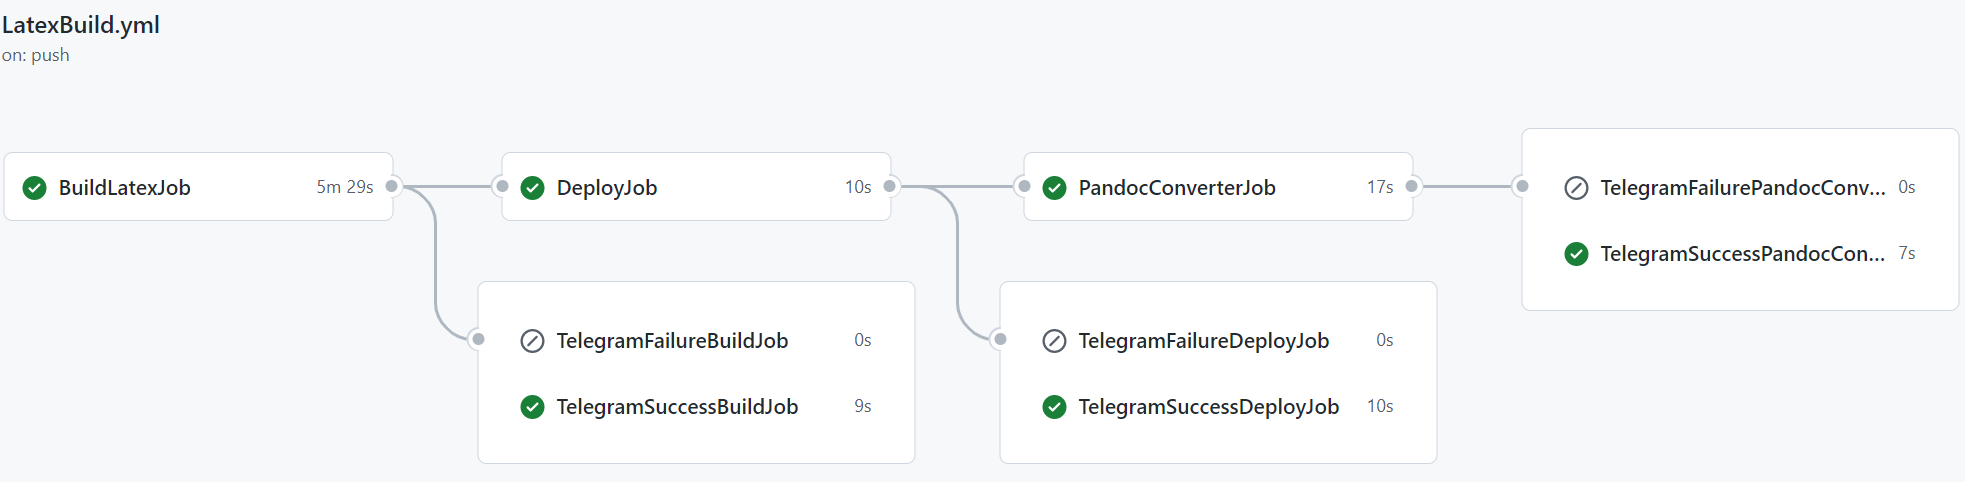
\includegraphics[width=1\textwidth]{Images/gh-pipeline.png}
        \end{figure}

        Qualora una persona volesse consultare la relazione online, senza scaricare il pdf, si è fatto uso di \textbf{Pandoc} per generare il relativo sito web, consultabile comodamente sul browser. Per la paginazione un template html/css è stato utilizzato per rendere la vista più accattivante.

        Il deploy del sito, infine, è stato utilizzato \textbf{GitHub-Pages} che permette di semplificarne la messa in opera avendo un branch dedicato sul quale tutti i file relativi possono essere mantenuti e aggiornati.
        

    \subsection{Progetto}
        \subparagraph{Tool utilizzati}
        \begin{itemize}
            \item Sbt
            \item ScalaTest
            \item GitHub Actions
            \item GitHub Pages
            \item Telegram Bots
            \item Dependabot
            \item Sonarcloud/Codacy/Codefactor
            \item Miro board
        \end{itemize}
    CI progetto, Test, Coverage, Documentazione, Quality assurance, bla bla
        








    % -*- root: ../main.tex -*-
\chapter{Analisi dello spazio del problema}

Inizialmente l'esperto del dominio è stato contattato per un'intervista preliminare (sotto riportata).
La sessione si è svolta in via telematica ed ha avuto lo scopo di prendere familiarità con l'ambito di lavoro e individuare i requisiti del software ad esso collegato. 
Nel colloquio il problema è emerso chiaramente e la soluzione software è stata individuata in maniera univoca.
In seguito sono stati definiti incontri periodici con il committente per la valutazione del progresso e i feedback sui deliverables di ogni sprint.

	\section{Intervista con il committente}
    
    Sono uno studente di Ingegneria e Scienze Informatiche dell'Università di Bologna presso la sede di Cesena. In questi anni ho dovuto studiare e ripassare la teoria per molti esami e ho trovato utile porre a me stesso delle domande alle quali dover rispondere, così da verificare la conoscenza della materia.
    In particolare, dopo aver acquisito una discreta quantità di nozioni, ho riscontrato la necessità di rivedere, in maniera generale, se riuscissi a ricordare i concetti principali per ogni topic dell'esame in questione.
    Per questo motivo, sarebbe utile poter avere a disposizione uno strumento che permetta di rendere più stimolante il ripasso pre esame. Ad esempio, vorrei non dover più scrivere su un foglio le domande e le relative risposte corrette e sbagliate. In più, vorrei poterle integrare con quelle dei miei compagni e viceversa, in modo da coprire il più possibile tutti gli argomenti di un esame. Vorrei anche potermi esercitare sulle domande che sbaglio più spesso, per migliorare le lacune. Trovo utile poter ripassare più materie contemporaneamente nei periodi di sessione, in cui ho più esami nella stessa settimana. Inoltre poter rispondere a più domande possibili nel minor tempo possibile, così da essere sicuro di riuscire a rispondere velocemente durante gli orali.
    
    
    \begin{QandA}
        \item Abbiamo pensato che il modo più divertente per poter studiare e ripassare potrebbe essere quello di fare un gioco a quiz, dove viene posta una domanda e quattro possibili risposte. Potrebbe essere utile?
            \begin{answered}
            Sarebbe molto interessante, così non mi annoierei. Metterei un'unica risposta corretta e le altre tre sbagliate. Ogni volta che ripasso una materia in particolare, le domande sono sempre le stesse? Perché a me piacerebbe rispondere correttamente attraverso il ragionamento, non solo ricordandomi a memoria la risposta data in precedenza.
            \end{answered}
        \item Per quanto riguarda il numero di domande per ogni argomento, abbiamo pensato di inserirne una quantità tale da avere sempre un ricambio adeguato ed evitare il ricircolo delle stesse. Inoltre anche le risposte saranno un numero superiore alle quattro visibili per ogni domanda.
        Quali modalità di gioco vorresti avere a disposizione?
            \begin{answered}
            Mi piacerebbe poter scegliere se rispondere a domande di uno specifico corso o di più corsi durante lo stesso quiz.
            \end{answered}
        \item Riguardo al tempo disponibile per rispondere, preferisce avere un tempo limite per ogni singolo quesito o per l'intera sessione di gioco?
            \begin{answered}
            Sicuramente vorrei avere un tempo limitato ad ogni domanda, per non incorrere nella tentazione di barare. Qualora fosse possibile avere anche una modalità di gioco con un tempo limite globale sarebbe molto divertente.
            \end{answered}
        \item Invece quali schermate di gioco vorresti visualizzare?
            \begin{answered}
            Dal menu principale vorrei poter scegliere le varie modalità di gioco, poter aggiungere ed esportare le domande e le risposte dei corsi e visualizzare le statistiche sulle partite effettuate in precedenza. Invece a fine partita vorrei visualizzare un riepilogo di tutte le domande presenti nel quiz appena concluso ed eventualmente, in caso di risposta errata, visualizzare la risposta corretta.
            \end{answered}
    \end{QandA}

    \newpage
    
    \section{Ubiquitous Language}
    Per chiarire il gergo usato tra il committente e gli sviluppatori è risultato essenziale adottare dei significati condivisi per i termini maggiormente usati. Ciò ha aiutato notevolmente anche la comunicazione tra gli sviluppatori stessi per non incorrere in malintesi.
    %TABELLA UBIQUITOUS LANGUAGE
    \begin{figure}[ht]
        \centering
        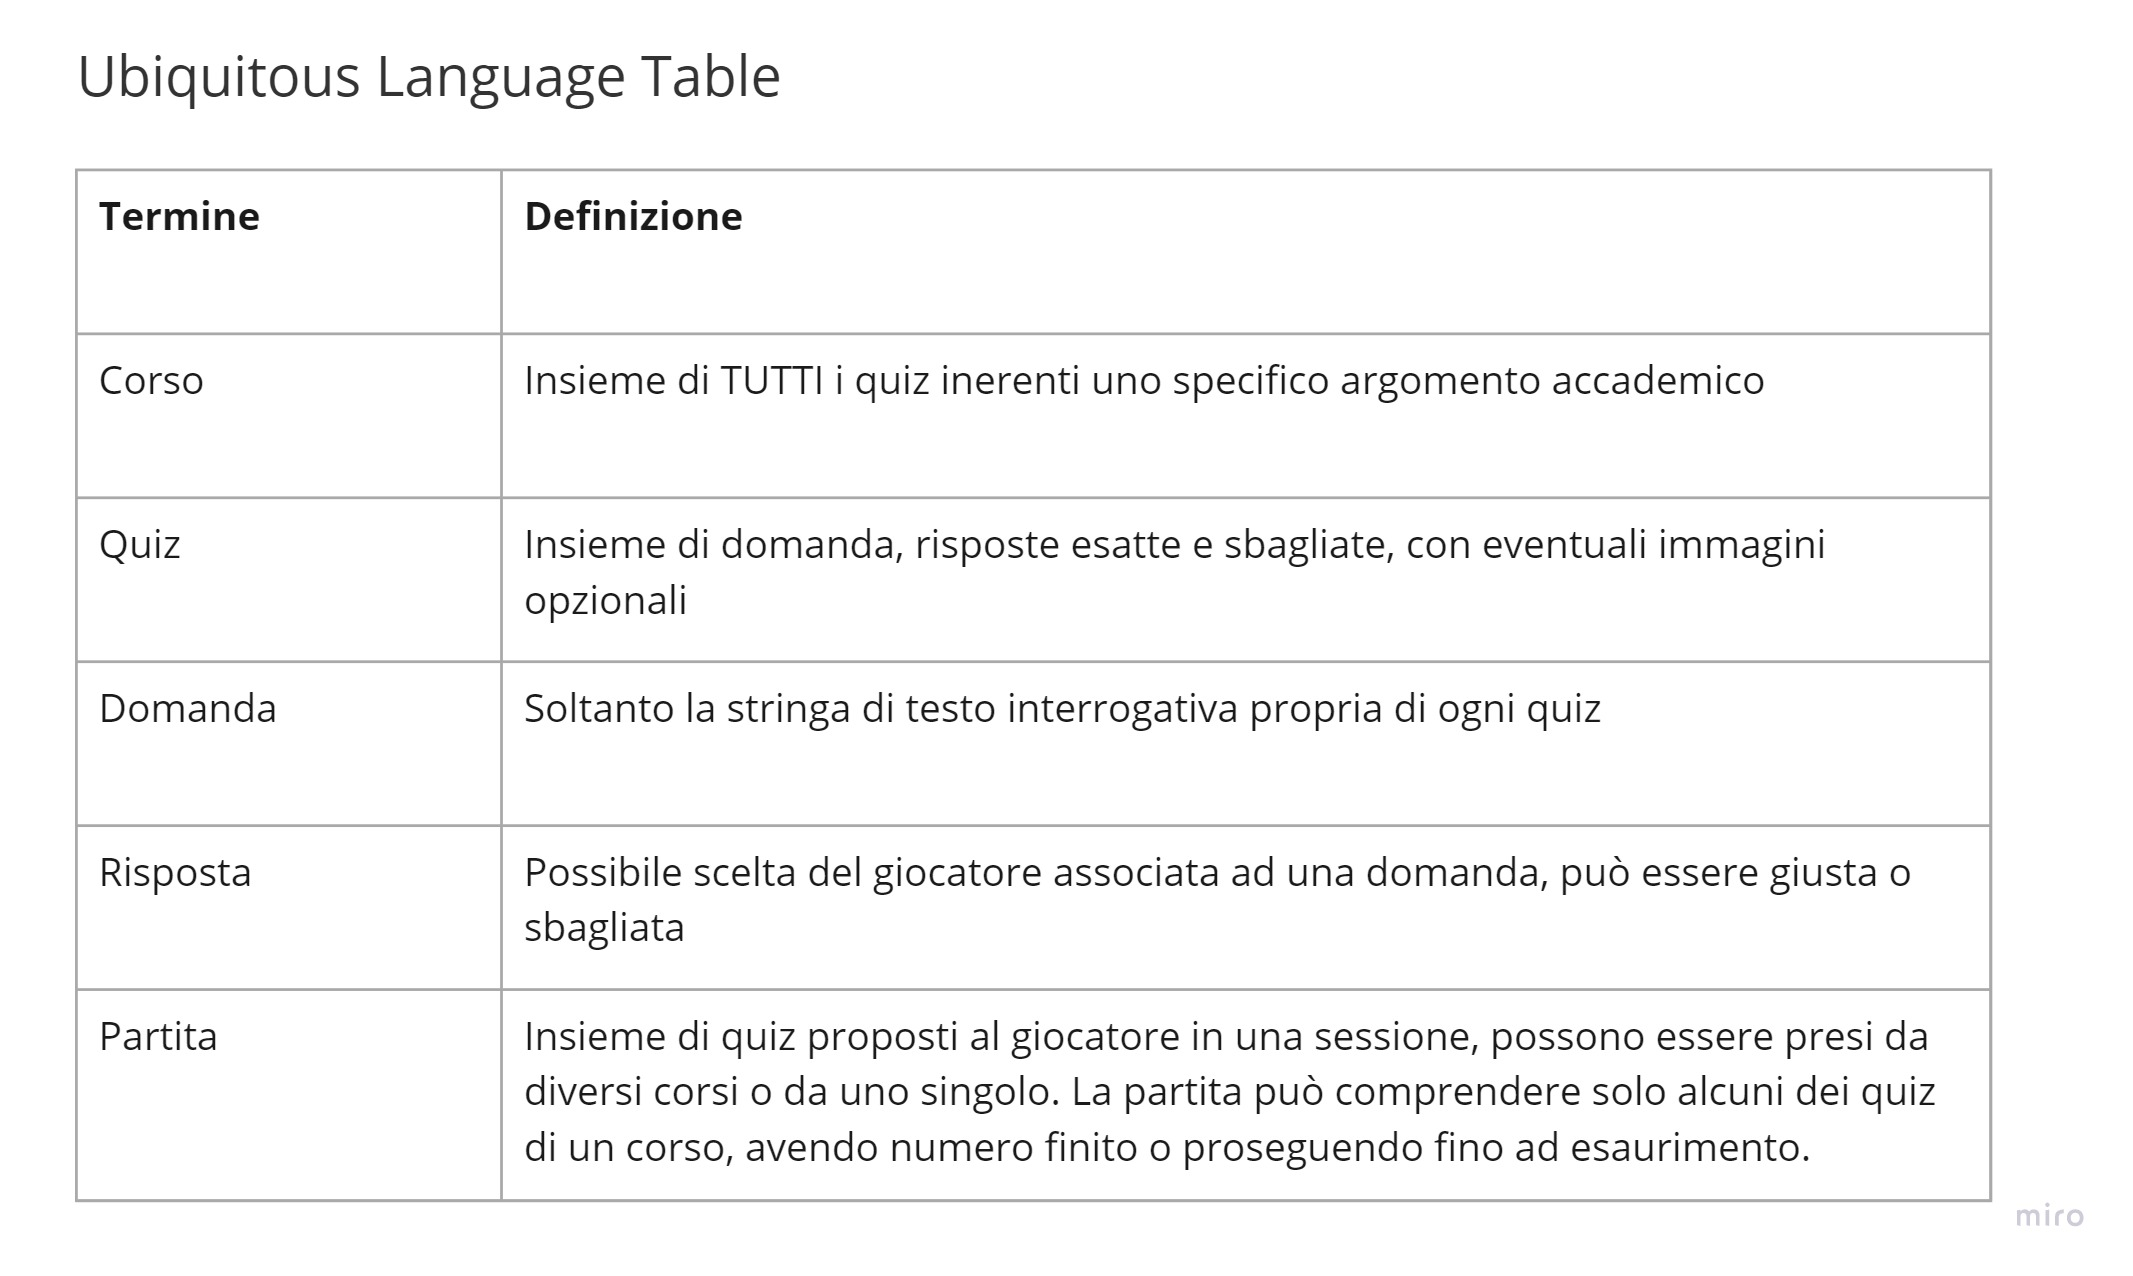
\includegraphics[width=0.9\textwidth]{Miro/ubiquitous-language.jpg}
        \caption{Tabella ubiquitous language}
        \label{fig:ubiquitouslanguage}
    \end{figure}
    % -*- root: ../main.tex -*-

% In questa sezione esporre brevemente i requisiti a cui il sistema proposto deve rispondere, concentrando l'attenzione sugli aspetti più rilevanti e facendo eventualmente uso di opportuni diagrammi di alto livello.
% 8000 - 10000 battute
% Attenzione in particolare ai requirement non funzionali: 1) non siano troppo vaghi altrimenti sono inverificabili, e quindi praticamente inutili; 2) se il sistema è distribuito, è inevitable dire cosa vi aspettate in termini di di robustezza a cambiamenti/guasti (quali?, come?), e scalabilità (in quale dimensione? fino a che punto?).

\chapter{Analisi dei Requisiti}
A seguito dell'intervista con l'esperto del dominio, sono emersi i seguenti requisiti per l'applicativo richiesto. Questi sono stati poi discussi e approvati dal committente.
\section{Requisiti di Business}
    L'importanza strategica del software risiede nel fornire agli studenti un valido strumento di ripasso e test delle competenze acquisite.
    Le aree semantiche di maggiore importanza sono l'interrogazione delle conoscenze tramite quesiti, il feedback sugli errori, la personalizzazione dei quiz, e delle statistiche globali e a fine partita. 
    I principali punti sono sotto riportati:
    \begin{itemize}
        \item selezione di N domande tra i C corsi scelti dell'utente
        \item gestione delle domande e delle relative risposte permettendo l'editing, il salvataggio e il caricamento delle stesse
        \item elaborare un riepilogo al termine di ogni partita
        \item elaborare e salvare alcune statistiche di interesse relativamente ad un utente
    \end{itemize}
	
\section{Requisiti Utente}
    Uno user dell'applicazione dovrà quindi essere in grado di:
    \begin{itemize}
        \item ripassare: visualizzare domande e scegliere tra le possibili risposte
        \item scegliere tra varie modalità di gioco
        \item visualizzare un riepilogo a fine partita
        \item visualizzare le proprie statistiche su tutte le partite effettuate
        \item importare ed esportare nuove domande e risposte indicando la materia a cui si riferiscono
    \end{itemize}
 
        \subsection{User Stories}
        \label{chap:UserStories}
        Si riportano di seguito le user stories emerse:
        \begin{itemize}
            \item Come utente voglio poter accedere all'applicativo e far iniziare una nuova partita;
            \item Come utente voglio poter selezionare la risposta che ritengo corretta, ricevendo un feedback a riguardo;
            \item Come utente voglio poter visualizzare le statistiche personali;
            \item Come utente voglio poter selezionare i corsi prima dell'inizio di ogni partita;
            \item Come utente voglio poter selezionare la modalità di gioco;
            \item Come utente voglio poter cambiare le impostazioni di gioco;
            \item Come utente voglio poter aggiungere domande, qualora volessi integrare nuovi quiz;
            \item Come utente voglio poter modificare domande aggiunte, qualora non siano corrette;
            \item Come utente voglio poter importare le domande in blocco relative a uno o più esami;
            \item Come utente voglio poter esportare le domande in blocco relative a uno o più esami;
            \item Come utente voglio poter riguardare i quiz della partita appena terminata.
        \end{itemize}
        
        \begin{figure}[H]
            \centering
            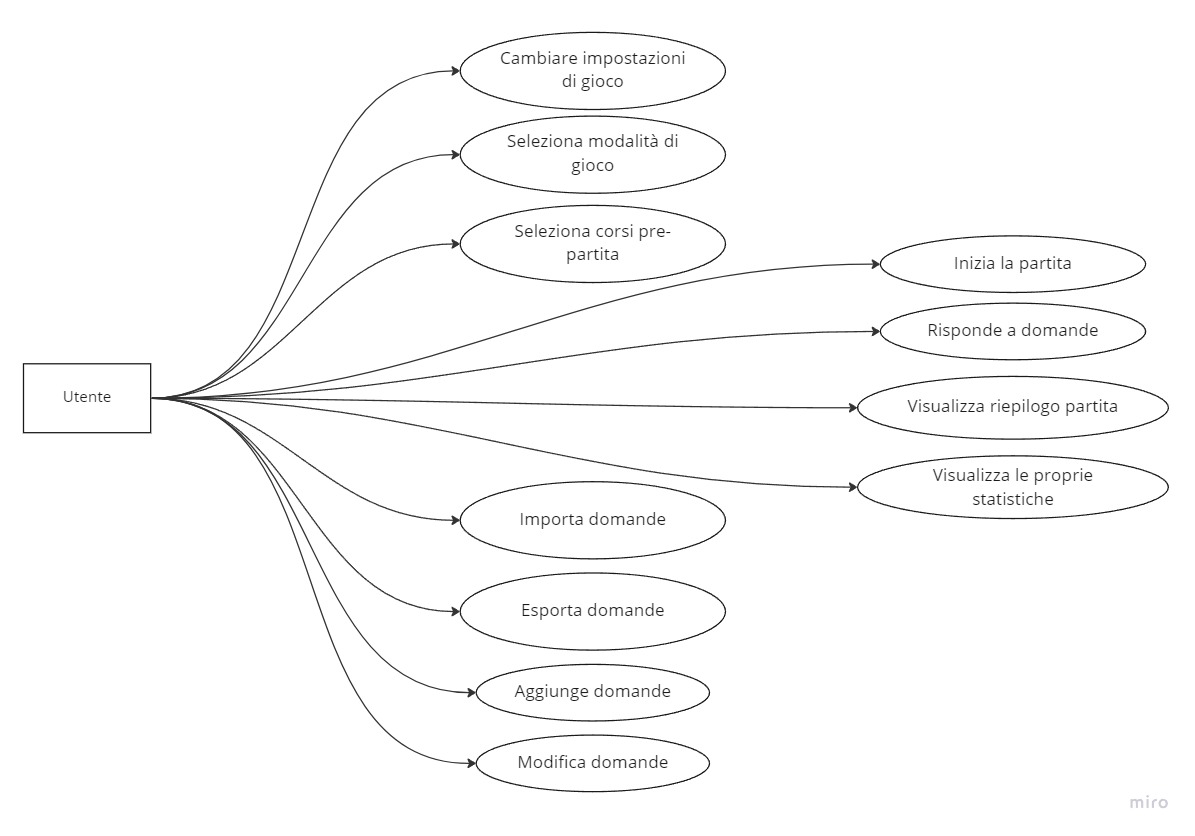
\includegraphics[width=\textwidth]{Miro/use-case.jpg}
            \caption{Schema Casi d'Uso}
            \label{fig:use-case}
        \end{figure}

        \subsection{Mockup}
        \label{chap:Mockup}
    	A seguito dell'intervista fatta con l'esperto del dominio e dei requisiti raccolti con esso, il team di sviluppo ha prodotto due versioni di mockup (\ref{mockup1} e \ref{mockup2}). In seguito, questi sono stati sottoposti al committente, il quale ha riscontrato aspetti positivi e negativi in entrambe le proposte. Di conseguenza, i mockup definitivi \ref{mockupFinished} sono stati sviluppati con la sua collaborazione e supervisione. Per garantire una maggior comprensione della navigazione all'interno dell'applicativo, è stato prodotto lo schema \ref{fig:mockup_nav}.
     
        \subsubsection{Mockup prima versione}\label{mockup1}
        
        \begin{figure}[H]
          \centering
          \begin{minipage}[b]{0.48\textwidth}
            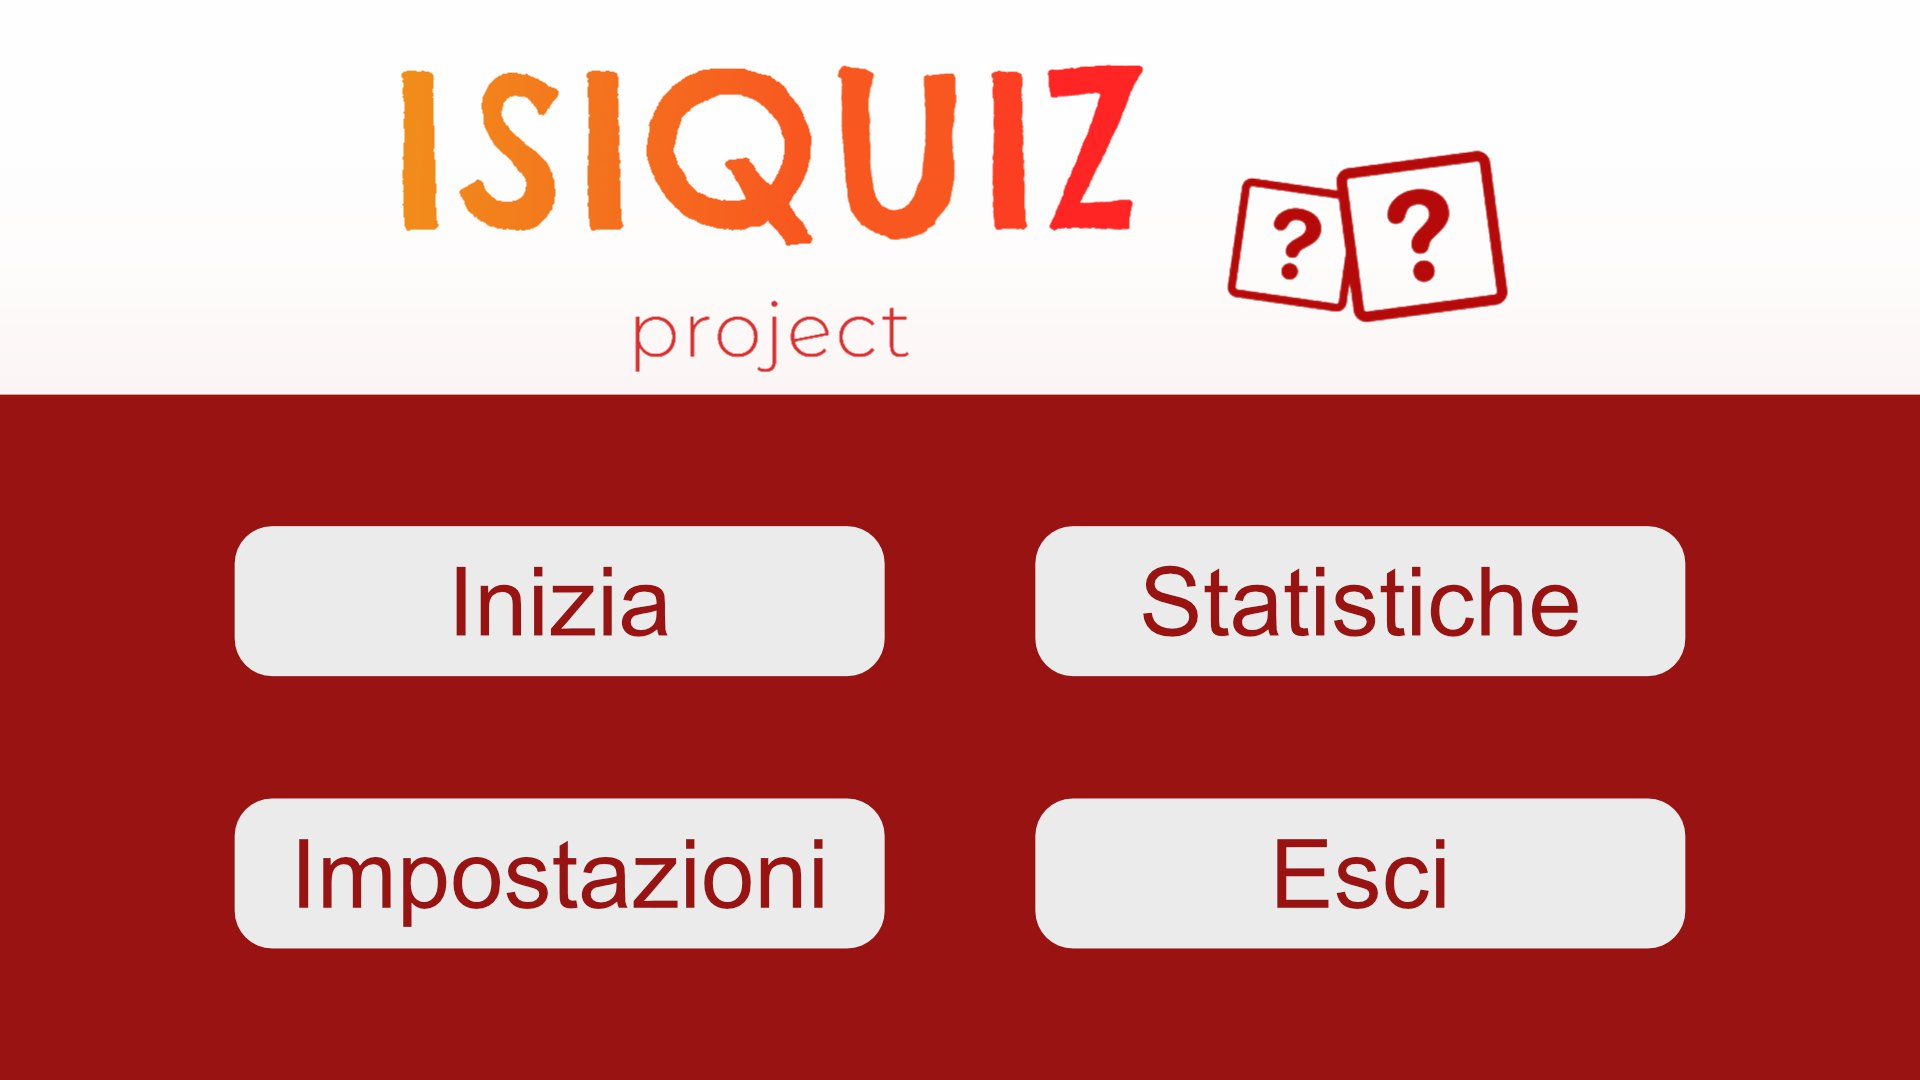
\includegraphics[width=\textwidth]{Images/mockup/home1.jpg}
            \caption{Pagina Iniziale}
            \label{fig:HomePage1}
          \end{minipage}
          \hfill
          \begin{minipage}[b]{0.48\textwidth}
            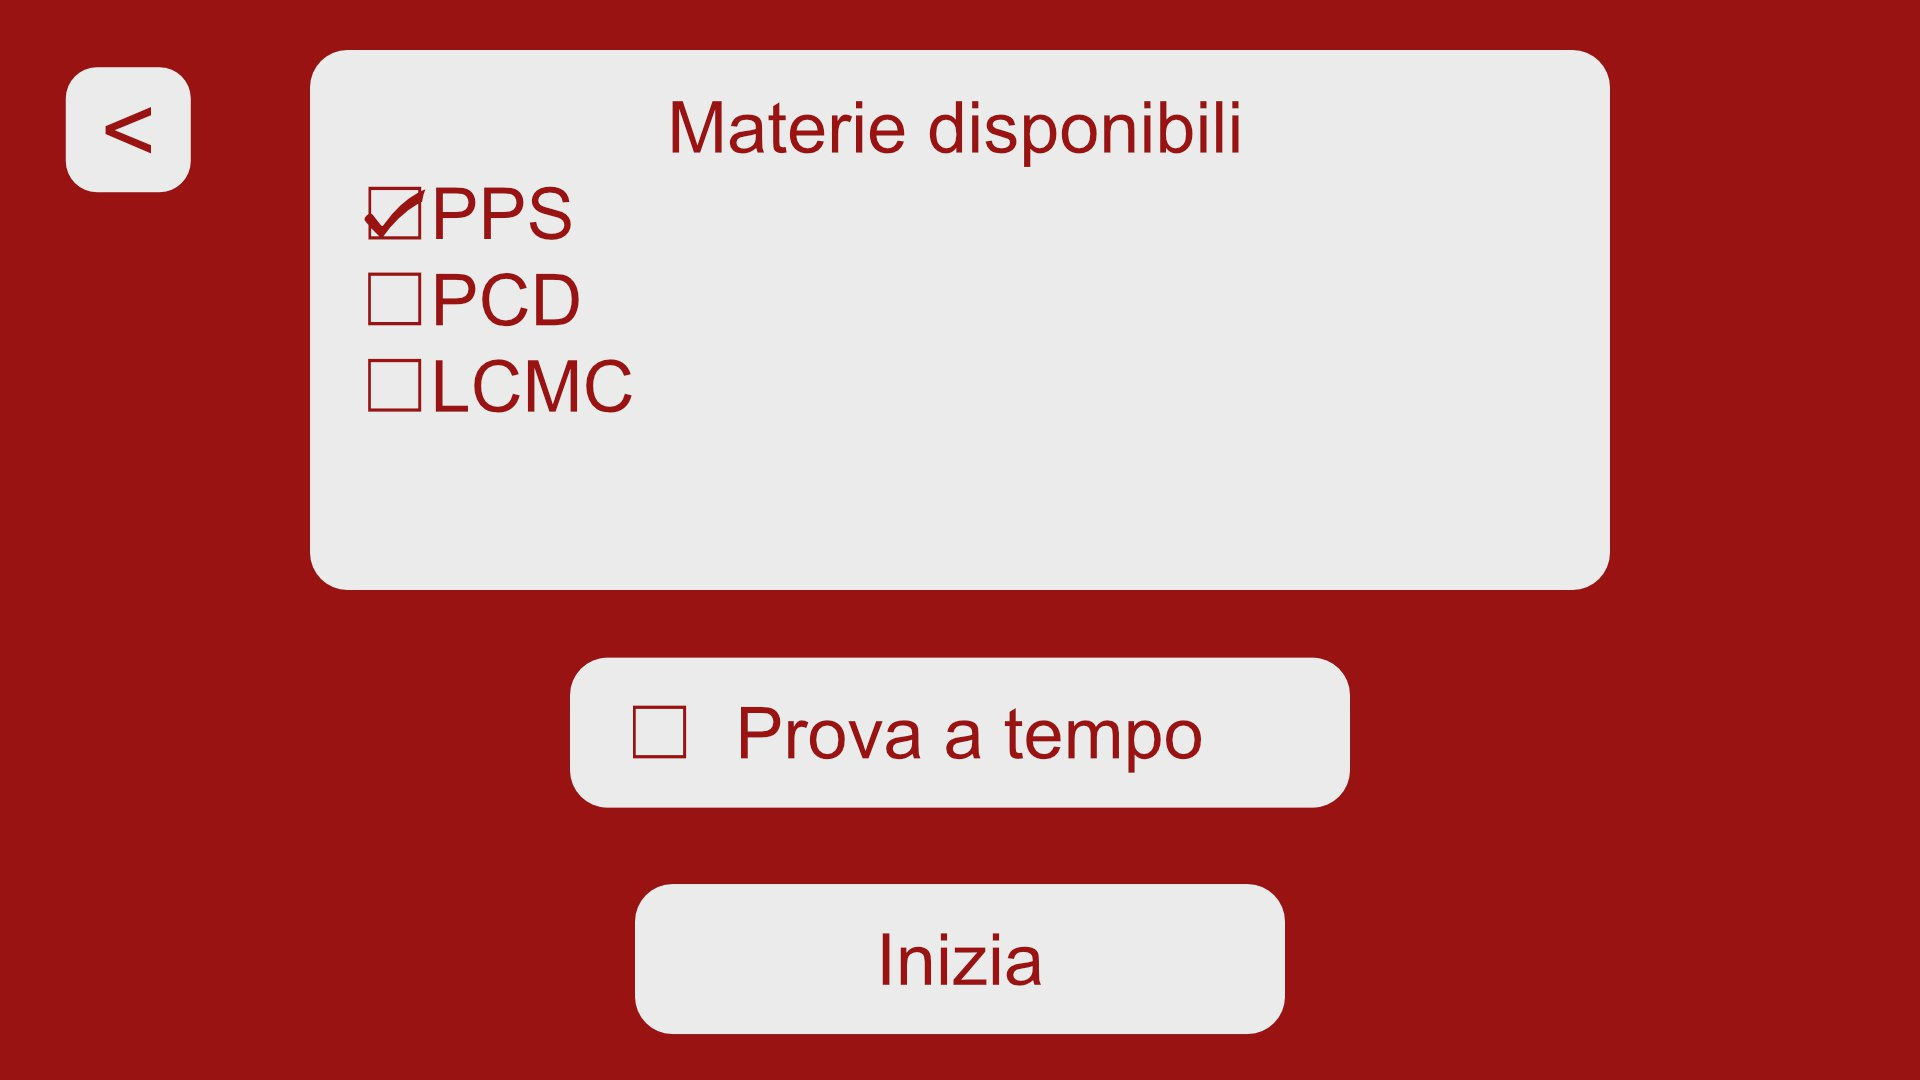
\includegraphics[width=\textwidth]{Images/mockup/start1.jpg}
            \caption{Settaggio di una partita prima di iniziarla}
            \label{fig:Start1}
          \end{minipage}
        \end{figure}

        \begin{figure}[H]
          \centering
          \begin{minipage}[b]{0.48\textwidth}
            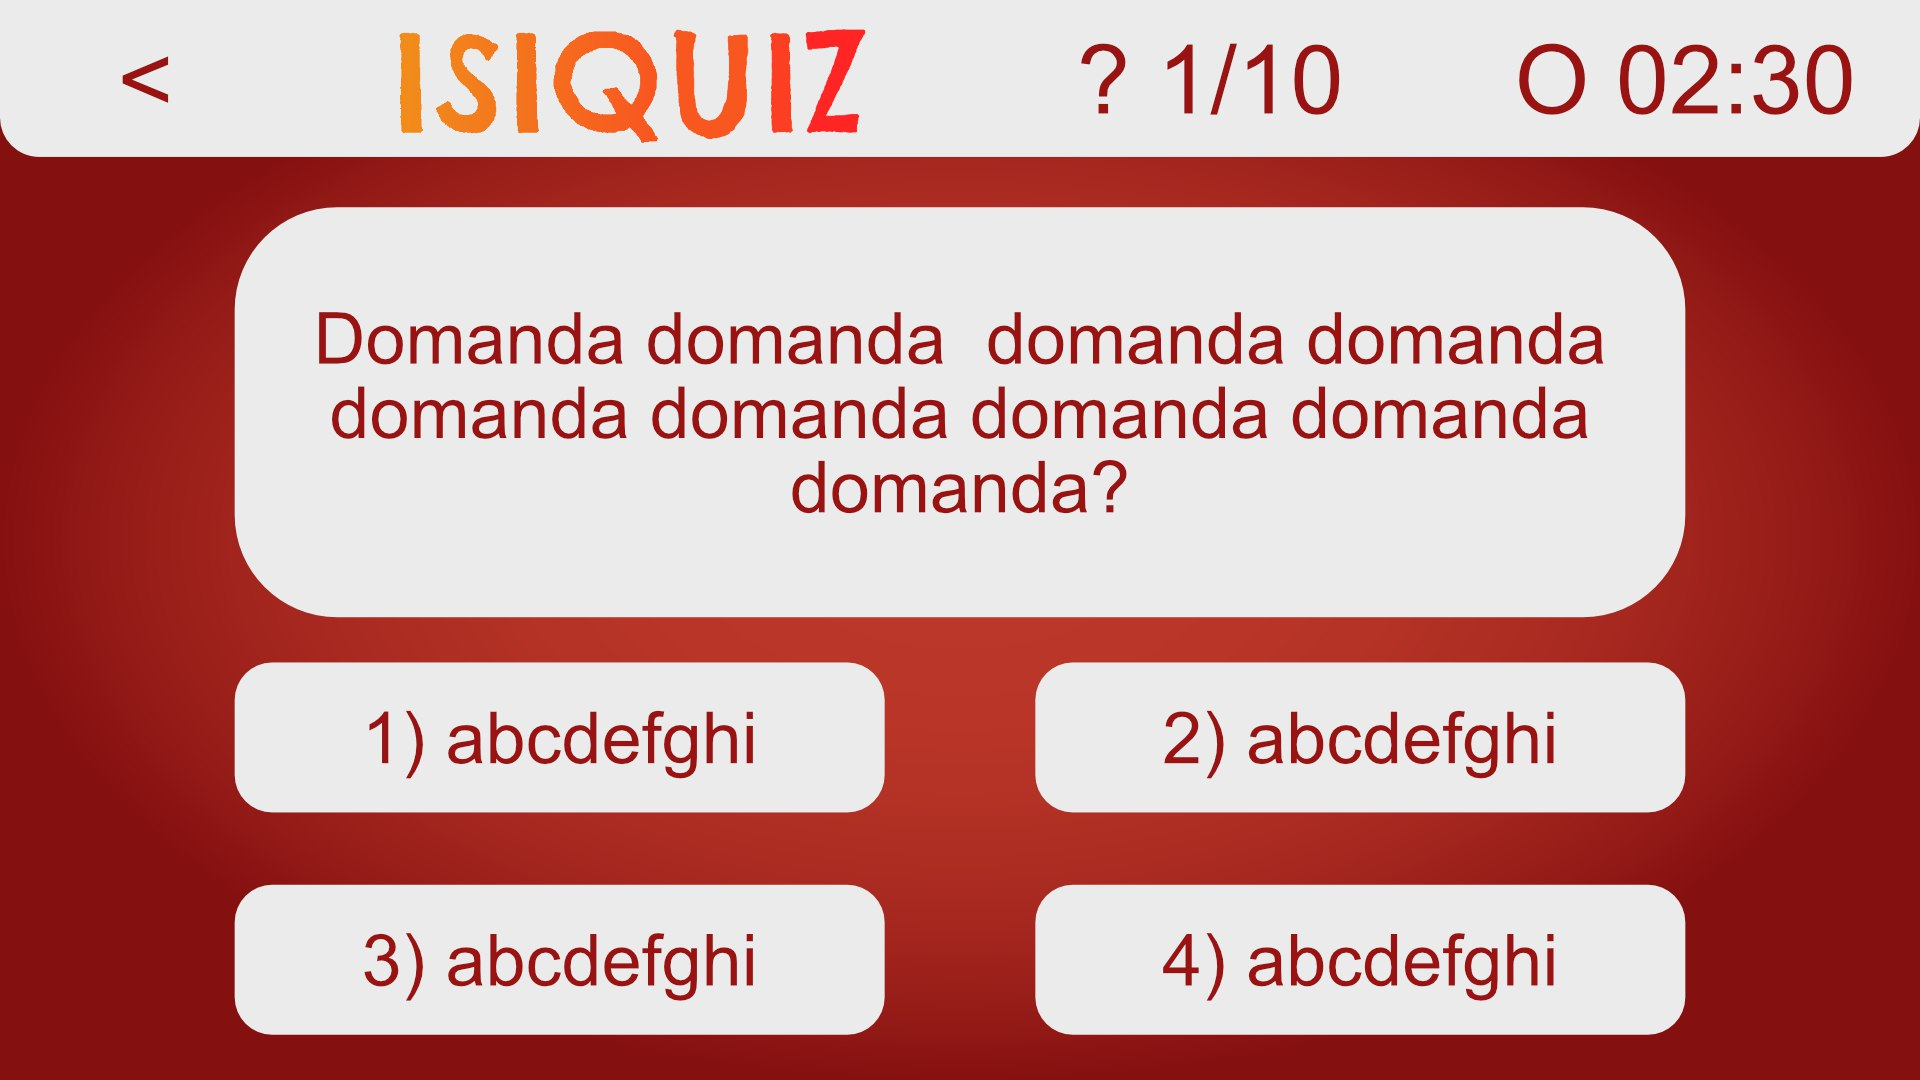
\includegraphics[width=\textwidth]{Images/mockup/quiz1.jpg}
            \caption{Quiz}
            \label{fig:Quiz1}
          \end{minipage}
          \hfill
          \begin{minipage}[b]{0.48\textwidth}
            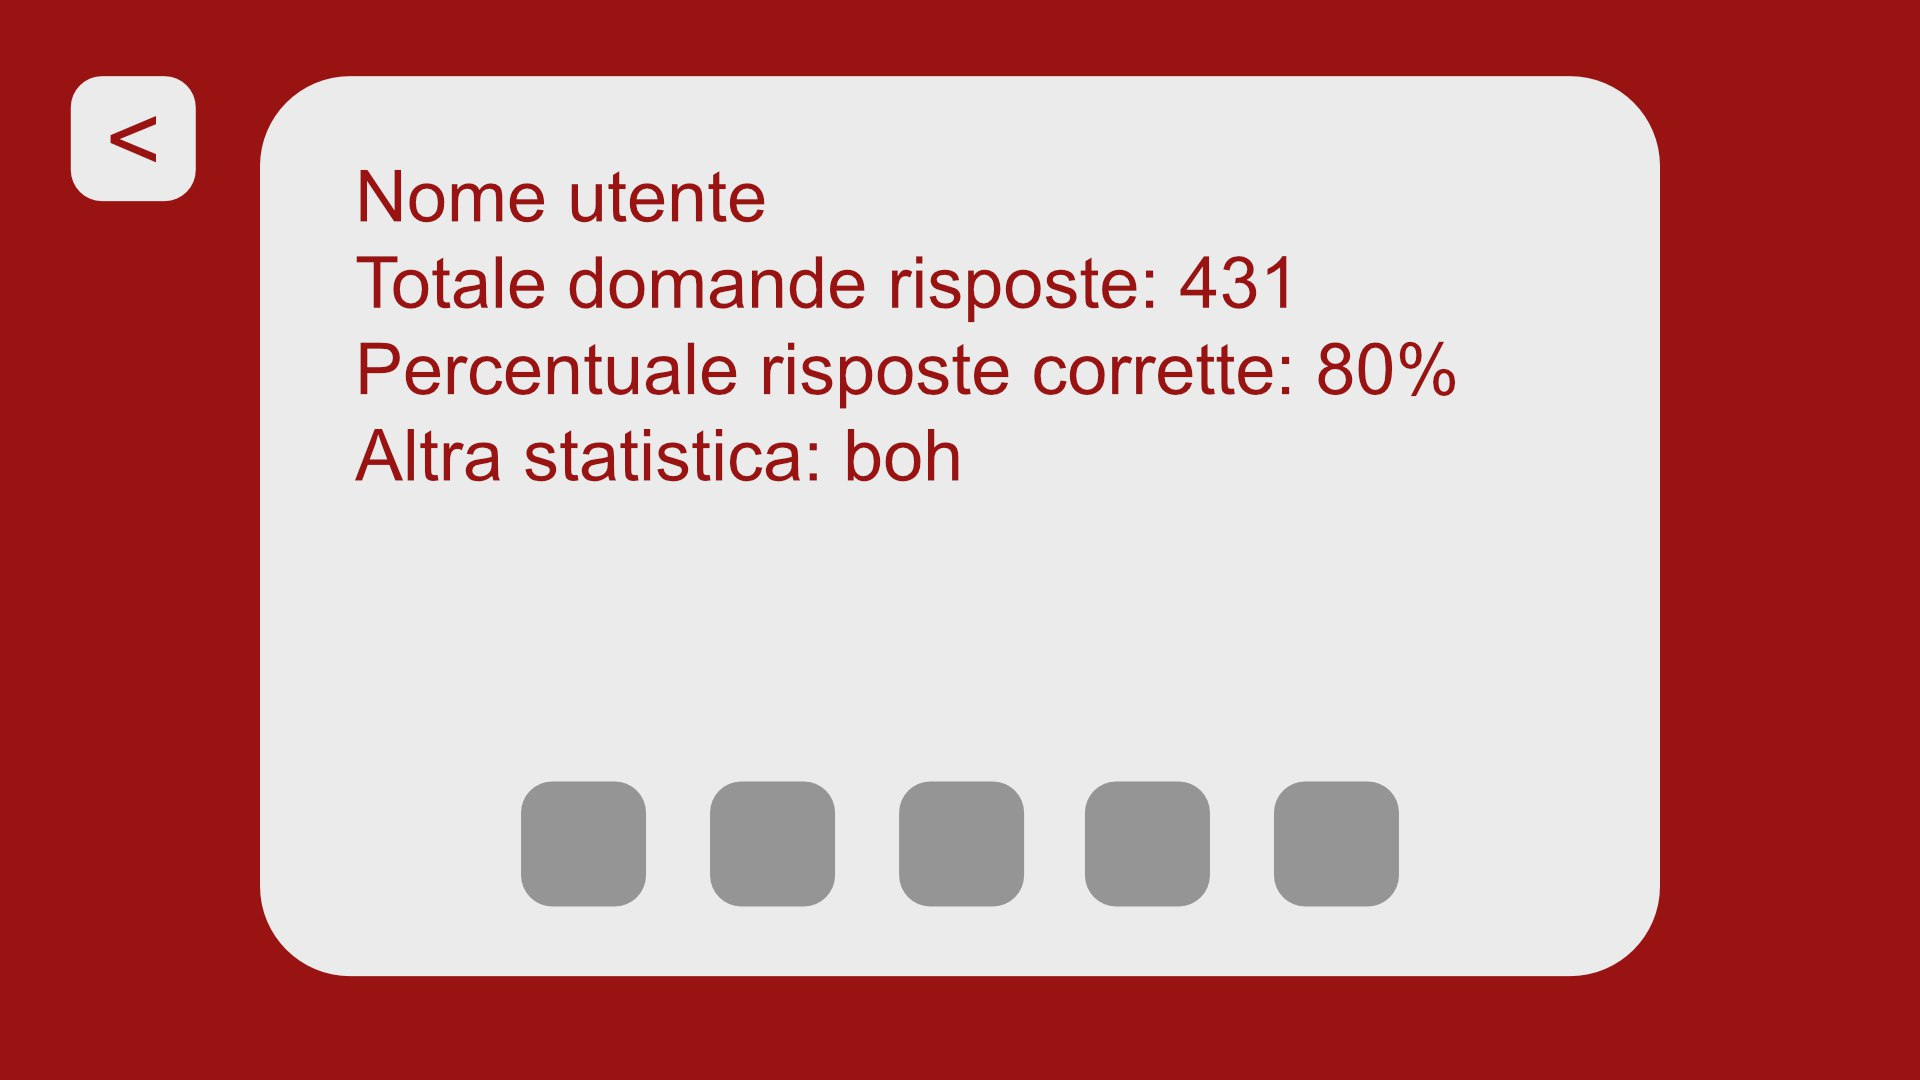
\includegraphics[width=\textwidth]{Images/mockup/achievements1.jpg}
            \caption{Statistiche di gioco e obiettivi raggiunti}
          \end{minipage}
        \end{figure}
          
        \begin{figure}[H]
          \centering
          \begin{minipage}[b]{0.48\textwidth}
            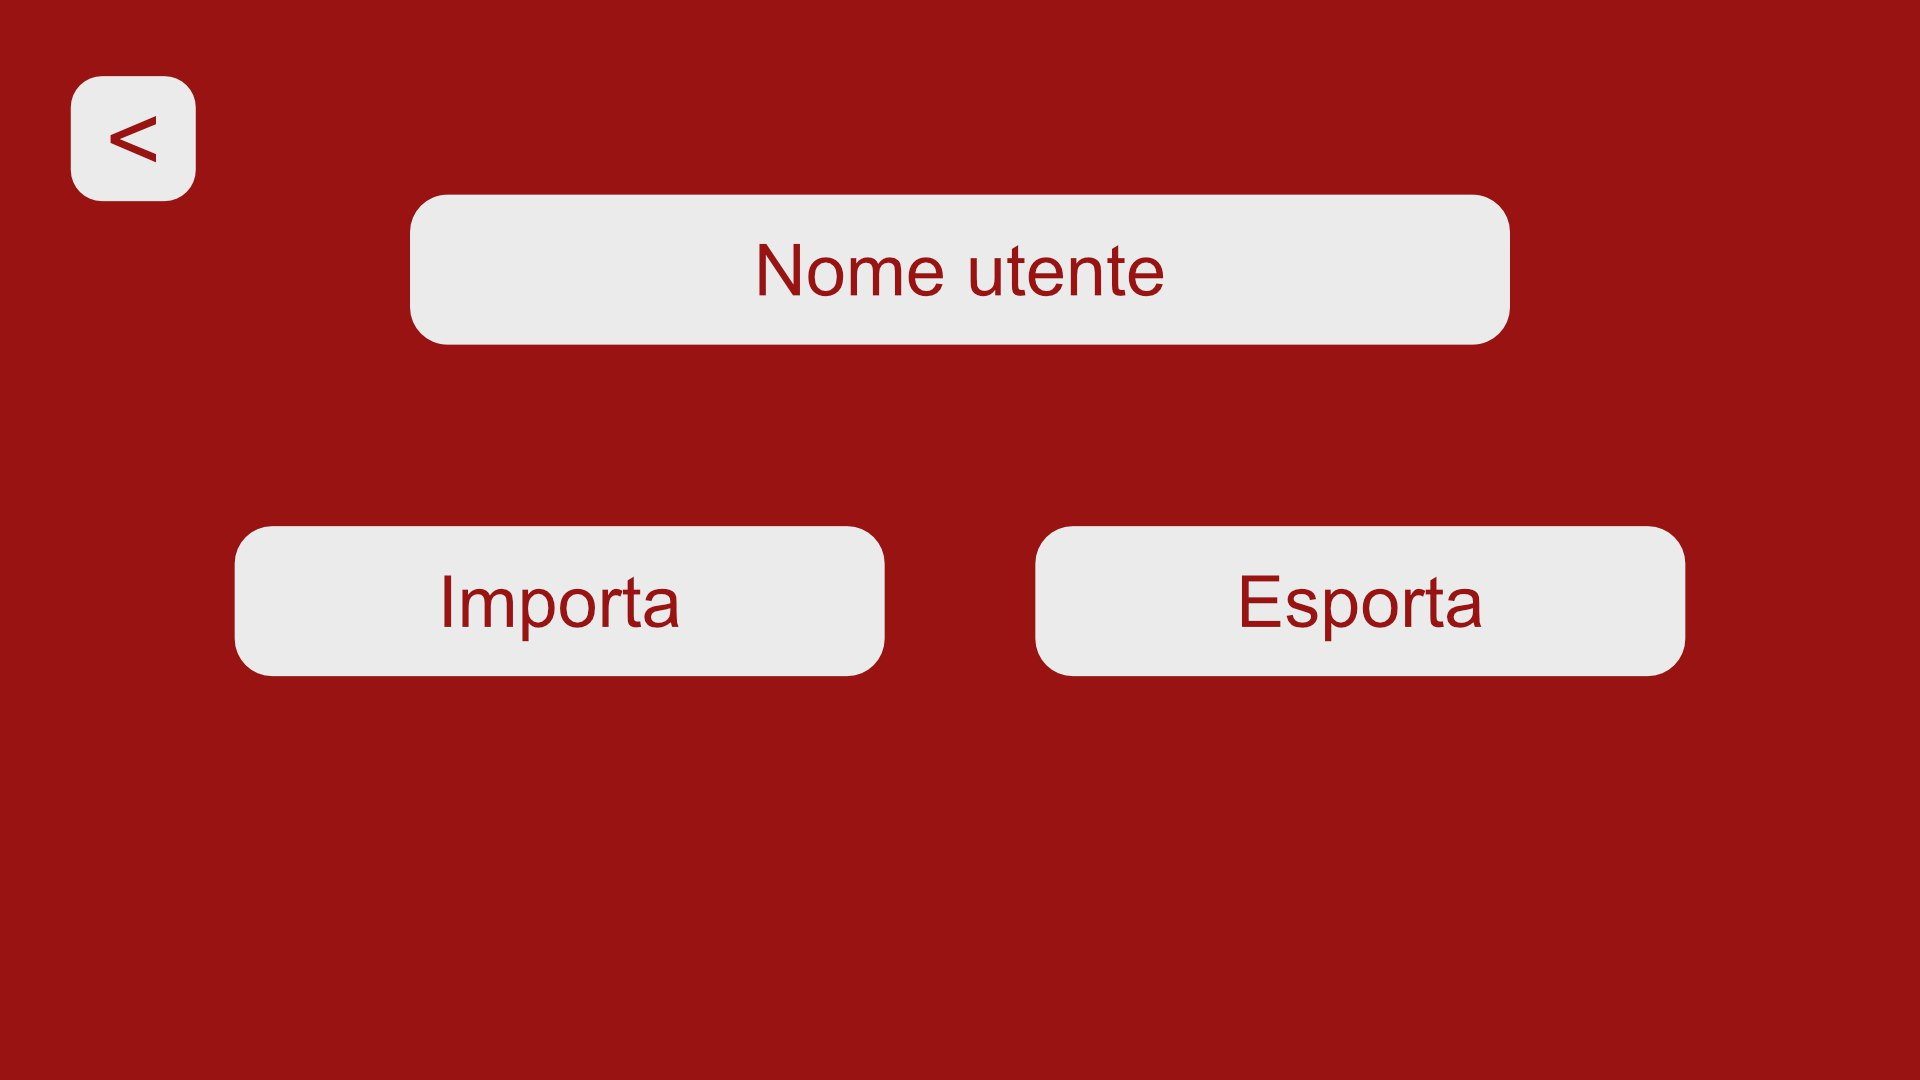
\includegraphics[width=\textwidth]{Images/mockup/settings1.jpg}
            \caption{Impostazioni Generali}
            \label{fig:Settings1}
          \end{minipage}
          \hfill
        \end{figure}
        
        \subsubsection{Mockup seconda versione}\label{mockup2}
        
        \begin{figure}[H]
          \centering
          \begin{minipage}[b]{0.48\textwidth}
            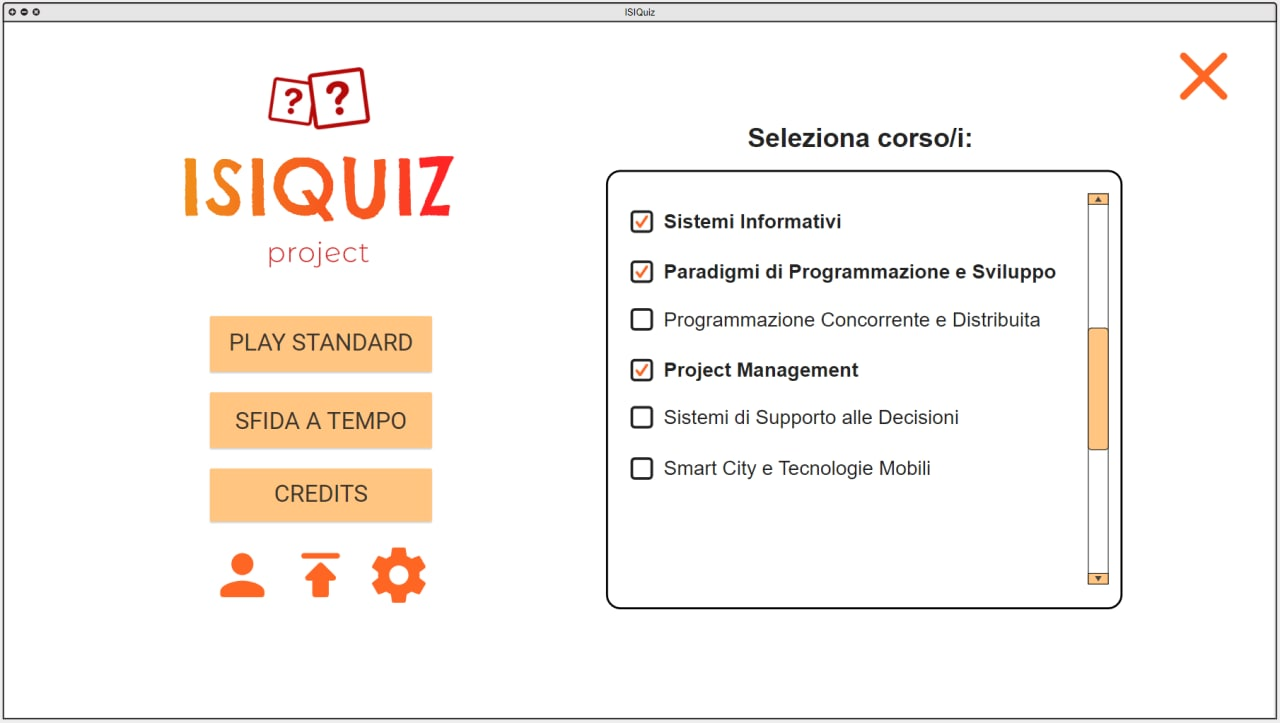
\includegraphics[width=\textwidth]{Images/mockup/home2.jpg}
            \caption{Pagina Iniziale}
            \label{fig:HomePage2}
          \end{minipage}
          \hfill
          \begin{minipage}[b]{0.48\textwidth}
            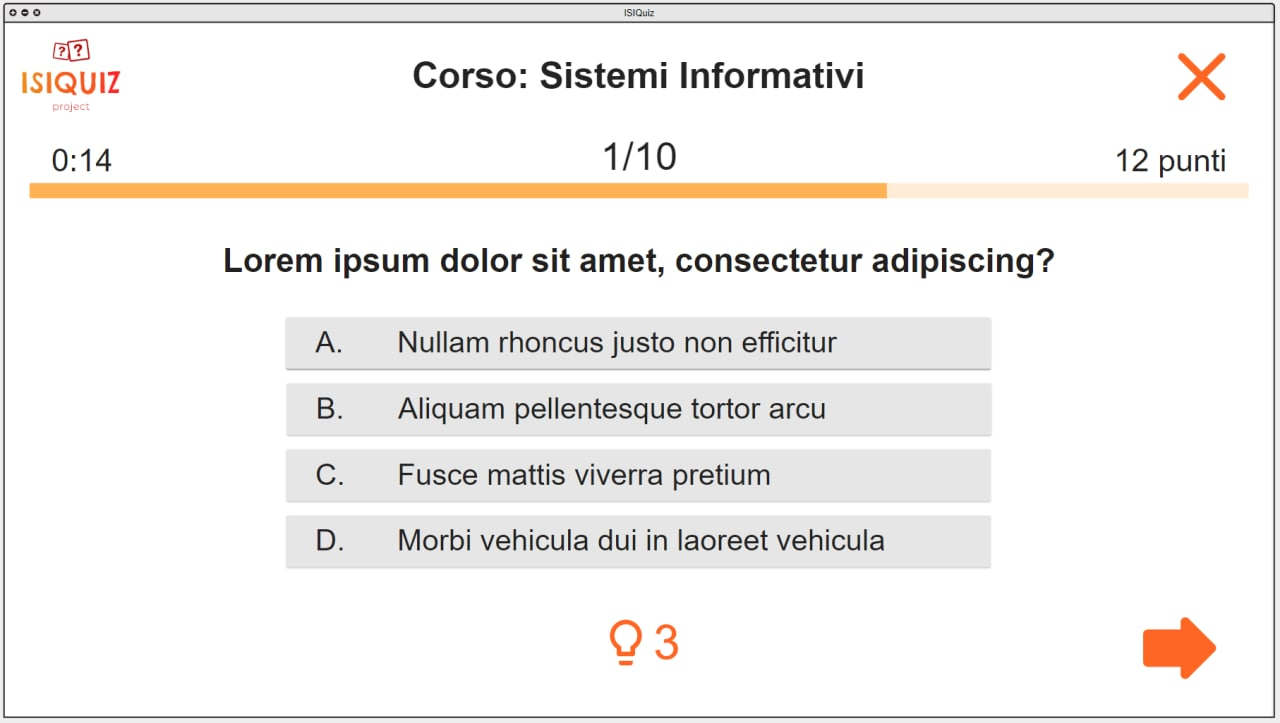
\includegraphics[width=\textwidth]{Images/mockup/quiz2.jpg}
            \caption{Quiz}
            \label{fig:Quiz2}
          \end{minipage}
        \end{figure}
          
        \begin{figure}[H]
          \centering
          \begin{minipage}[b]{0.48\textwidth}
            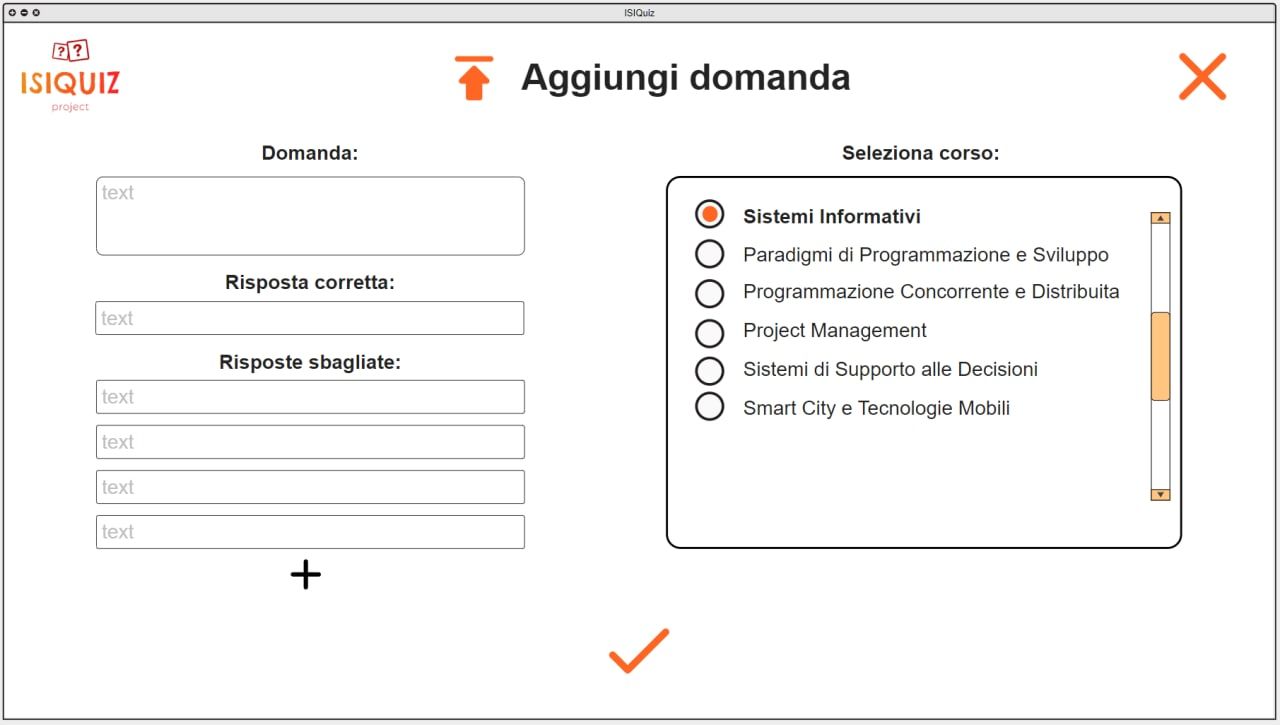
\includegraphics[width=\textwidth]{Images/mockup/import2.jpg}
            \caption{Inserimento di nuove domande e relative risposte per un determinato corso}
            \label{fig:Import2}
          \end{minipage}
          \hfill
        \end{figure}
        
        \subsubsection{Mockup definitivi}\label{mockupFinished}
        
        \begin{figure}[H]
          \centering
          \begin{minipage}[b]{0.48\textwidth}
            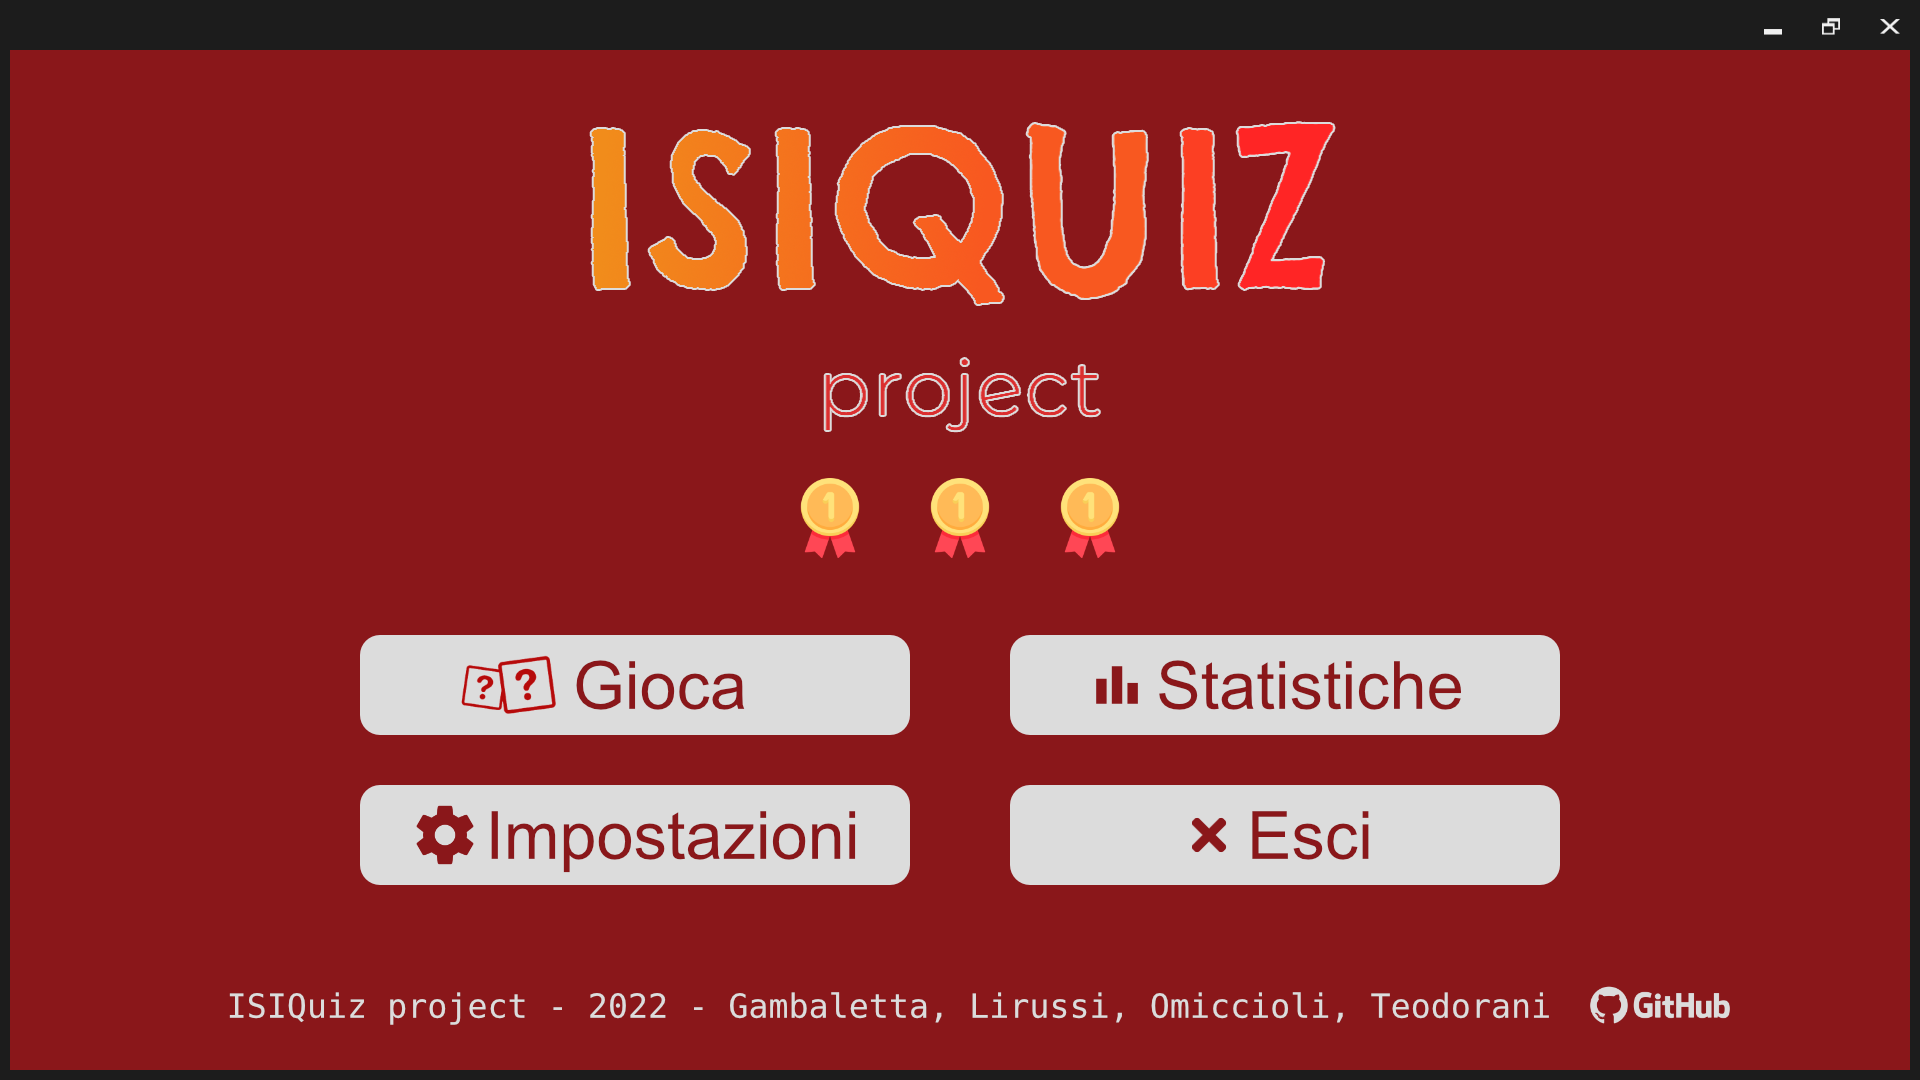
\includegraphics[width=\textwidth]{Images/mockup/home3.png}
            \caption{Pagina iniziale}
            \label{fig:home3}
          \end{minipage}
          \hfill
          \begin{minipage}[b]{0.48\textwidth}
            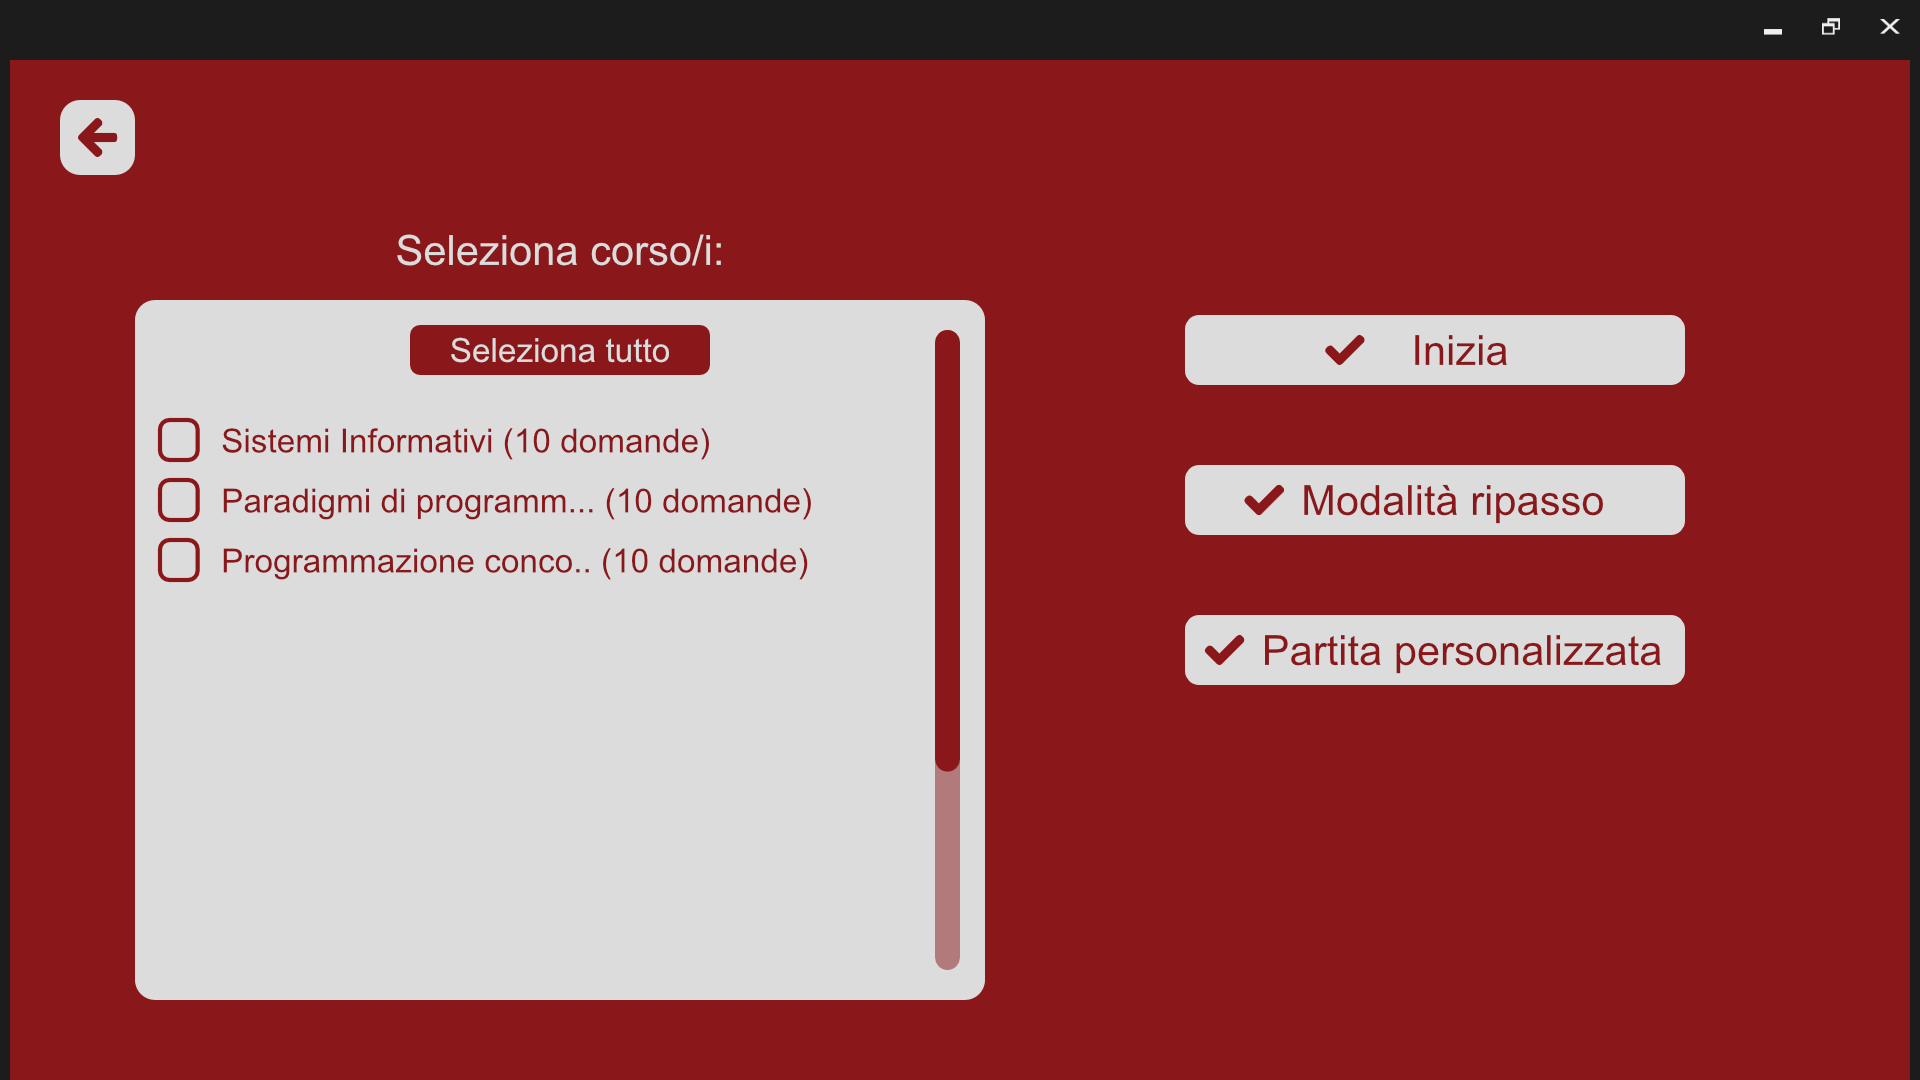
\includegraphics[width=\textwidth]{Images/mockup/start3.png}
            \caption{Settaggio di una partita prima di iniziarla}
            \label{fig:start3}
          \end{minipage}
        \end{figure}

        \begin{figure}[H]
          \centering
          \begin{minipage}[b]{0.48\textwidth}
            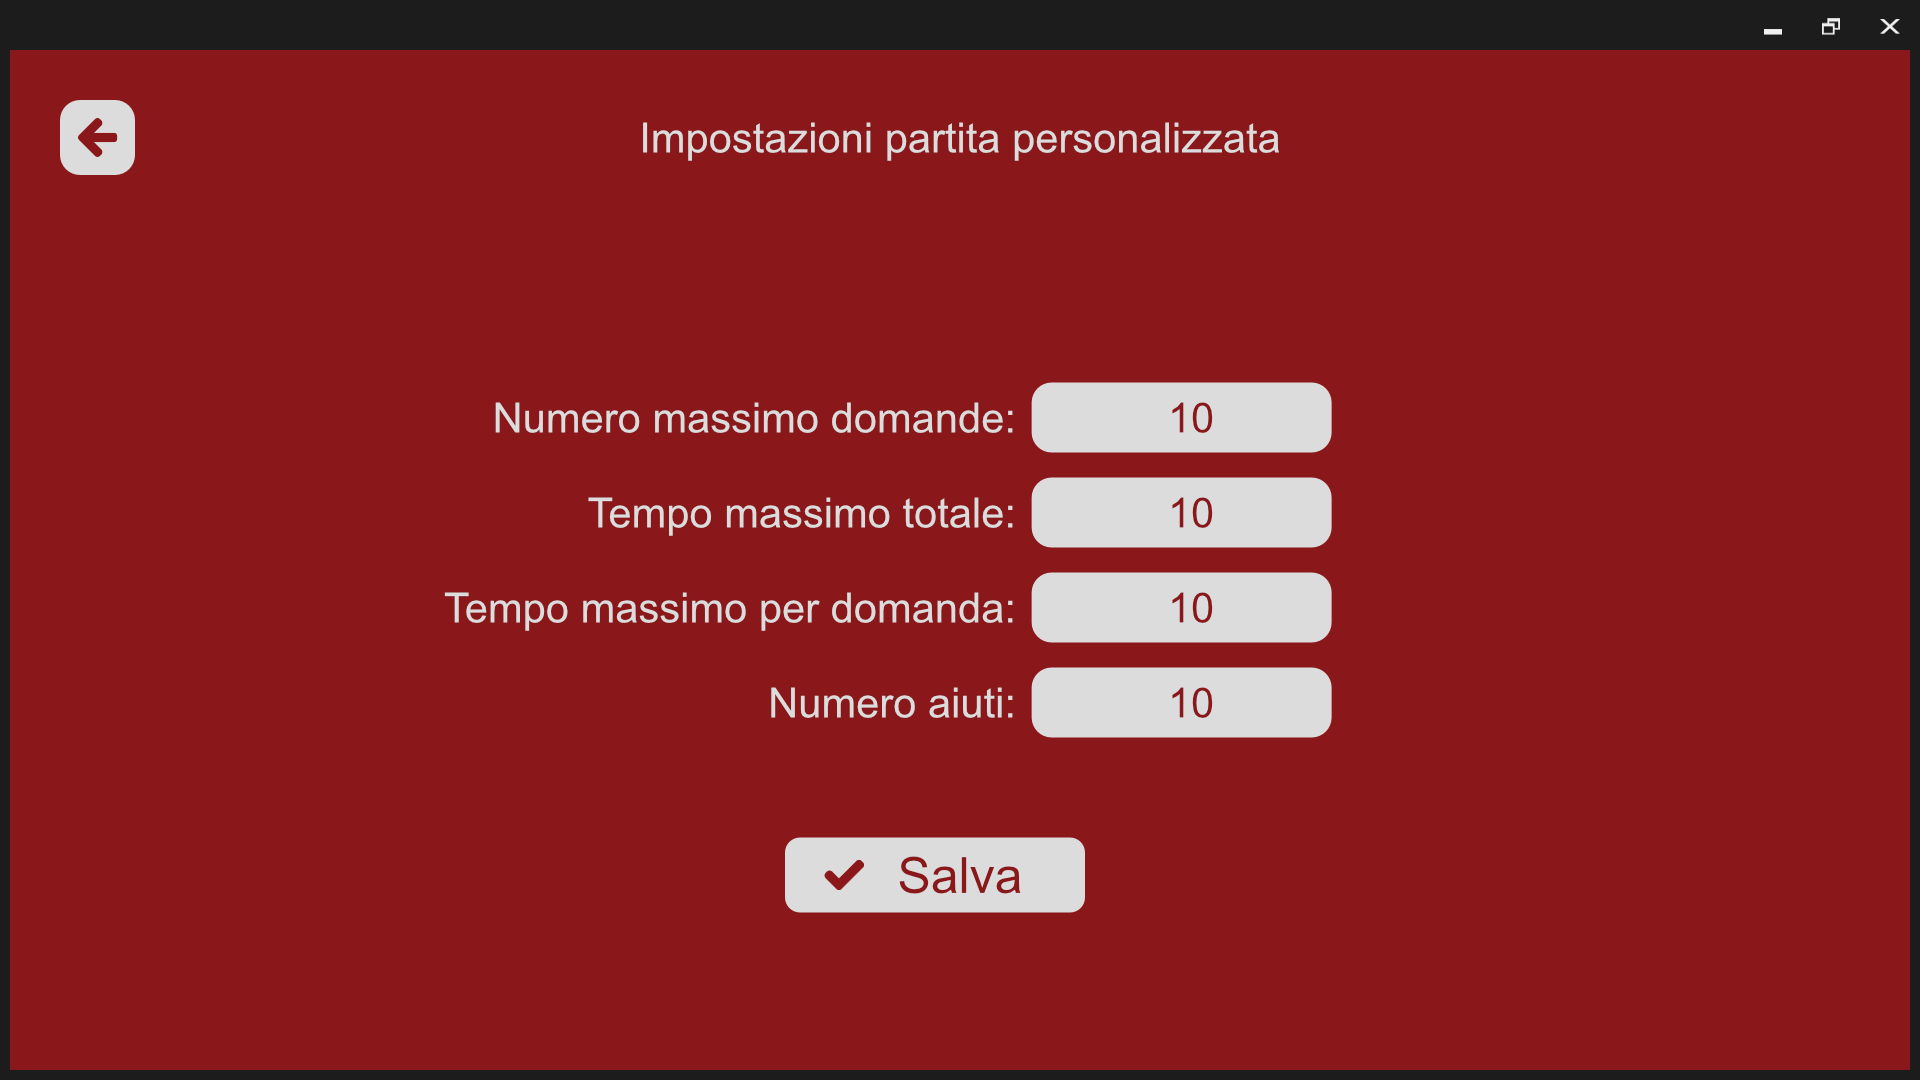
\includegraphics[width=\textwidth]{Images/mockup/custom.png}
            \caption{Settaggio parametri per una partita personalizzata}
            \label{fig:custom}
          \end{minipage}
          \hfill
          \begin{minipage}[b]{0.48\textwidth}
            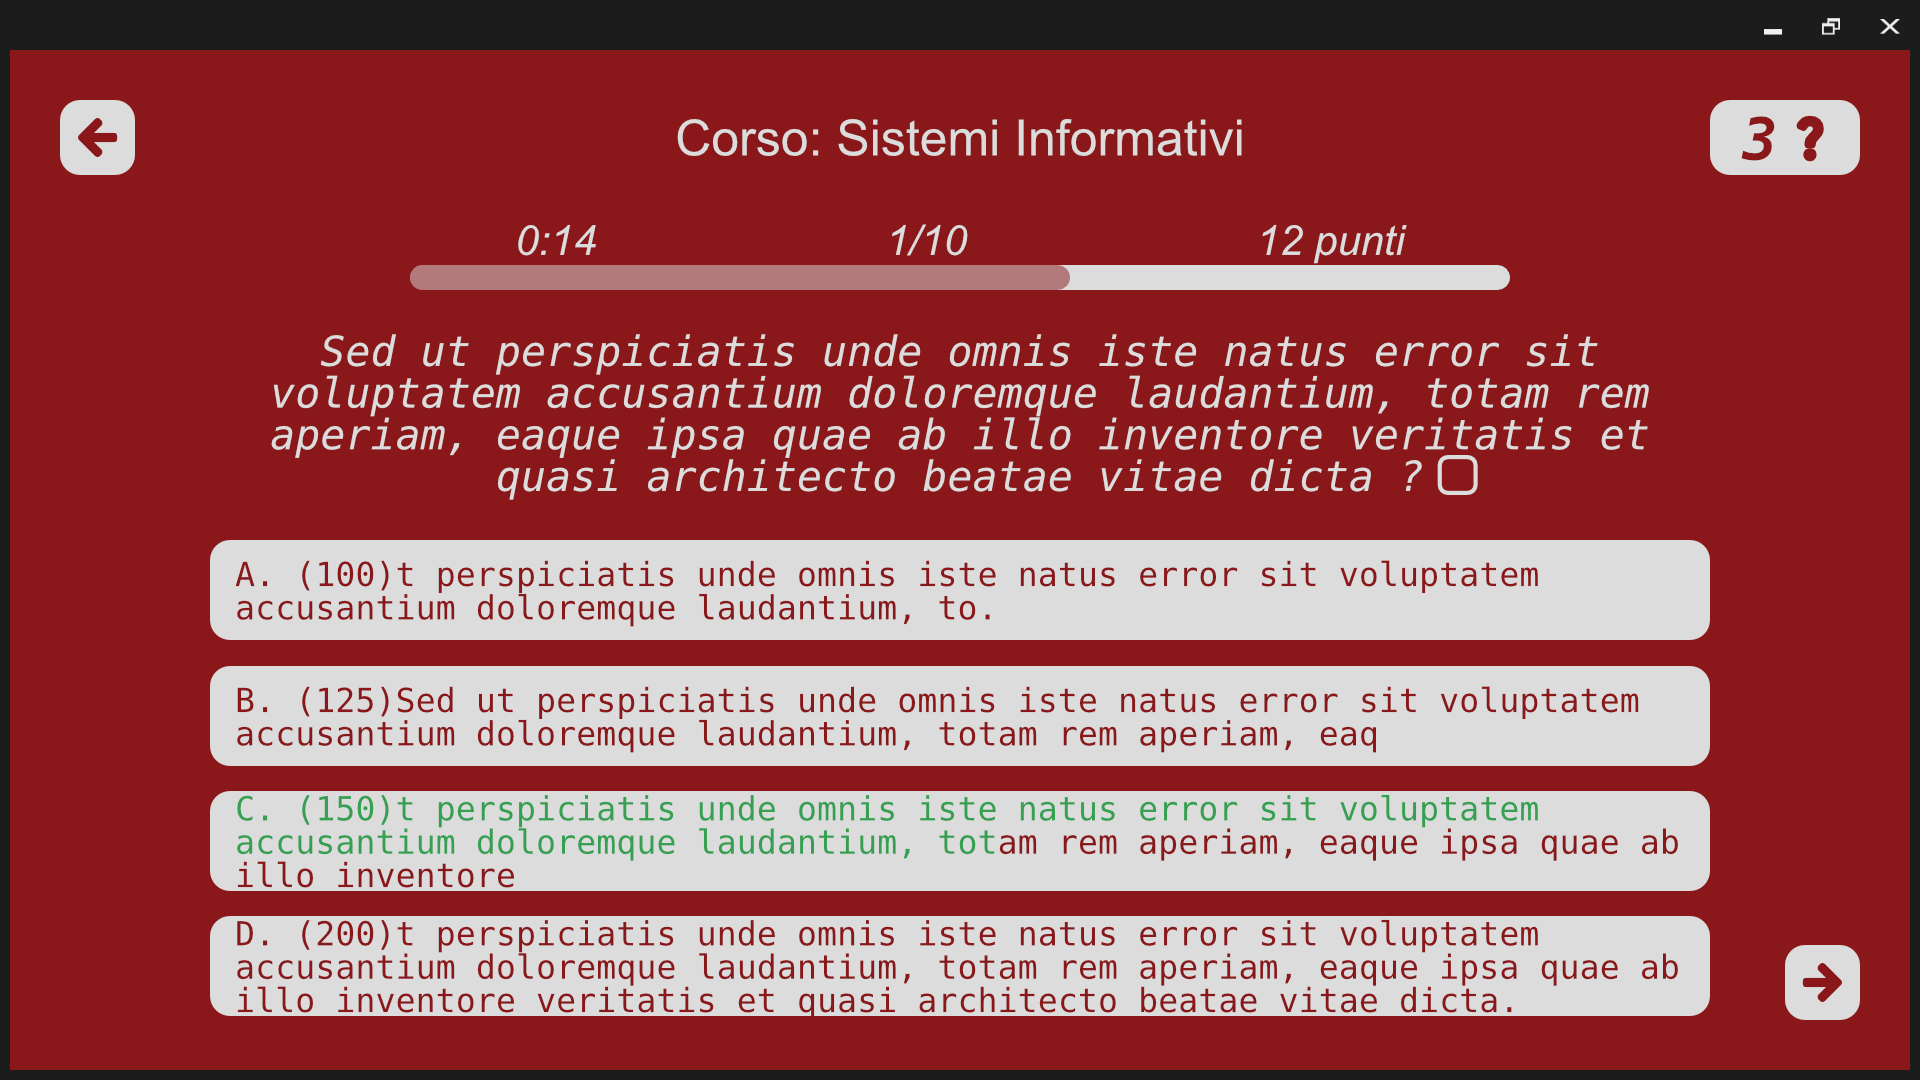
\includegraphics[width=\textwidth]{Images/mockup/quiz3.png}
            \caption{Quiz}
            \label{fig:quiz3}
          \end{minipage}
        \end{figure}

        \begin{figure}[H]
          \centering
          \begin{minipage}[b]{0.48\textwidth}
             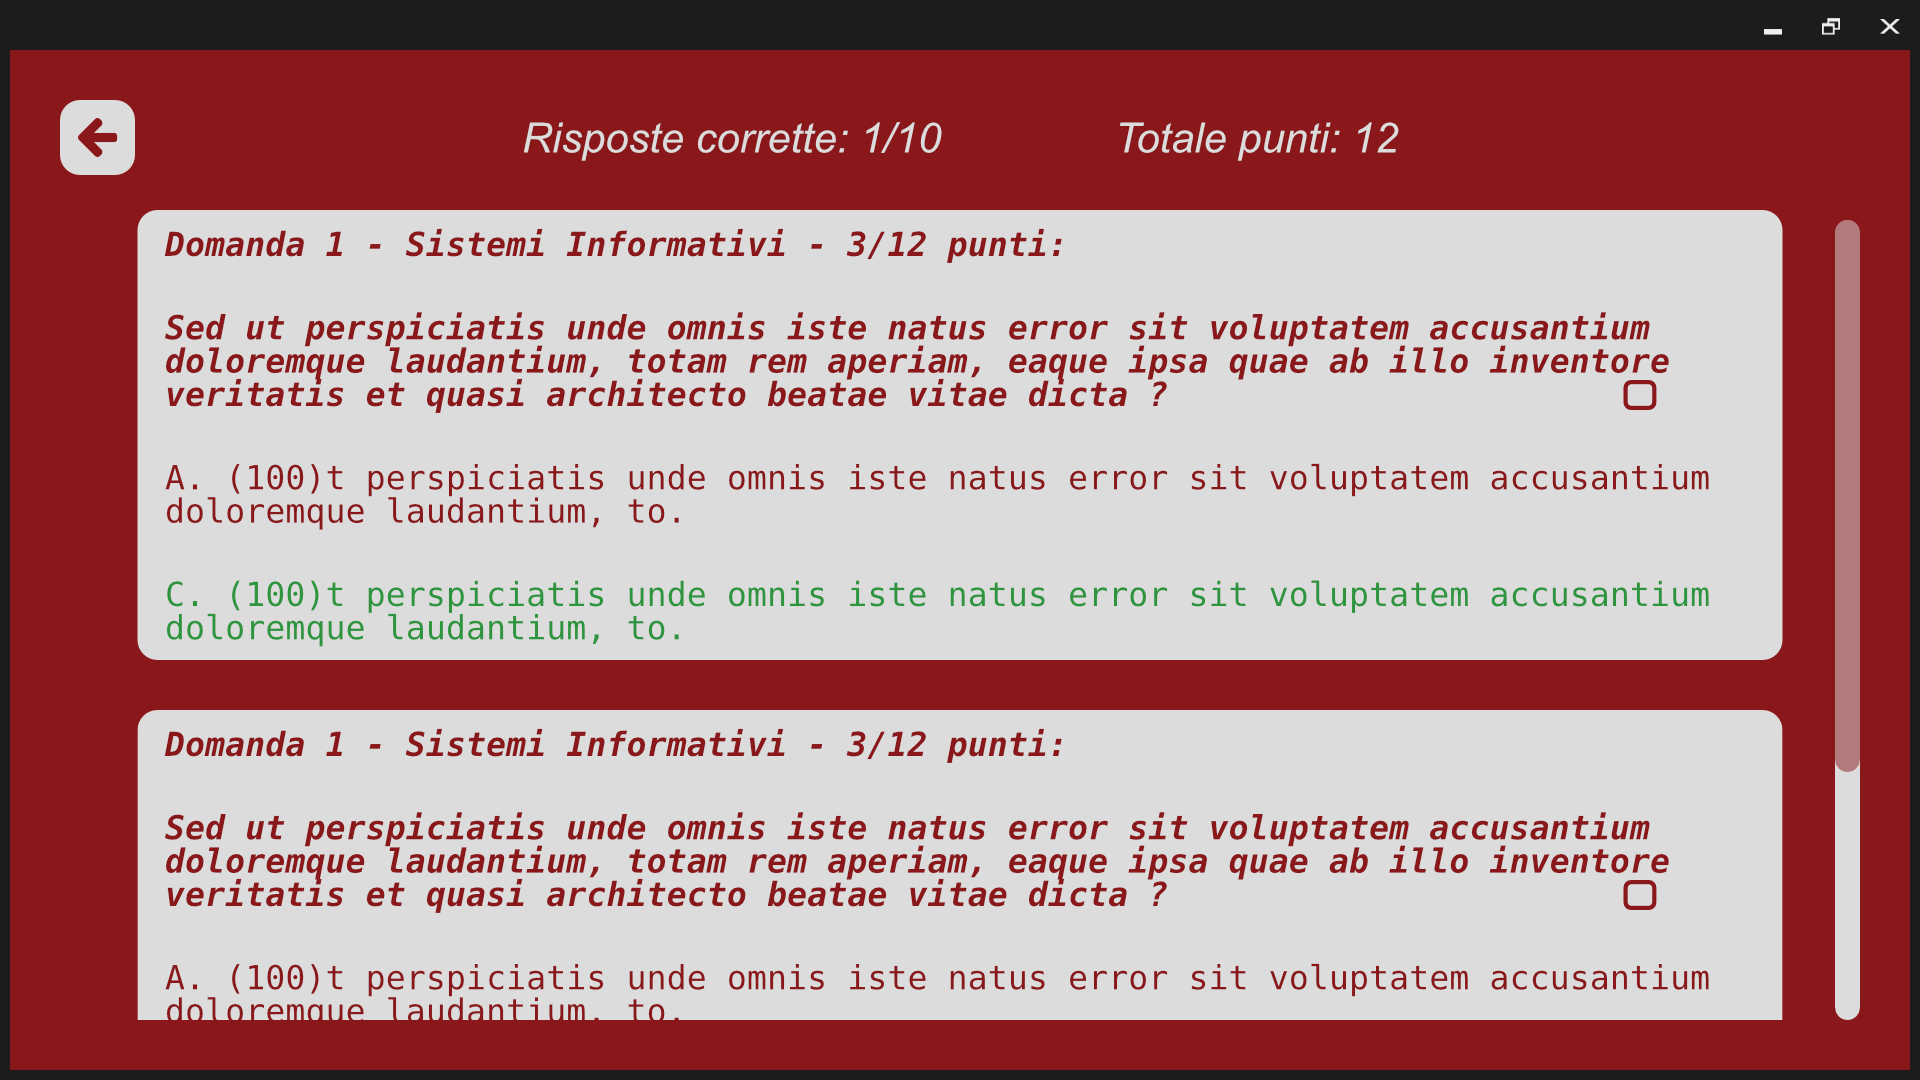
\includegraphics[width=\textwidth]{Images/mockup/review.png}
            \caption{Revisione al termine di un quiz}
            \label{fig:review}
          \end{minipage}
          \hfill
          \begin{minipage}[b]{0.48\textwidth}
            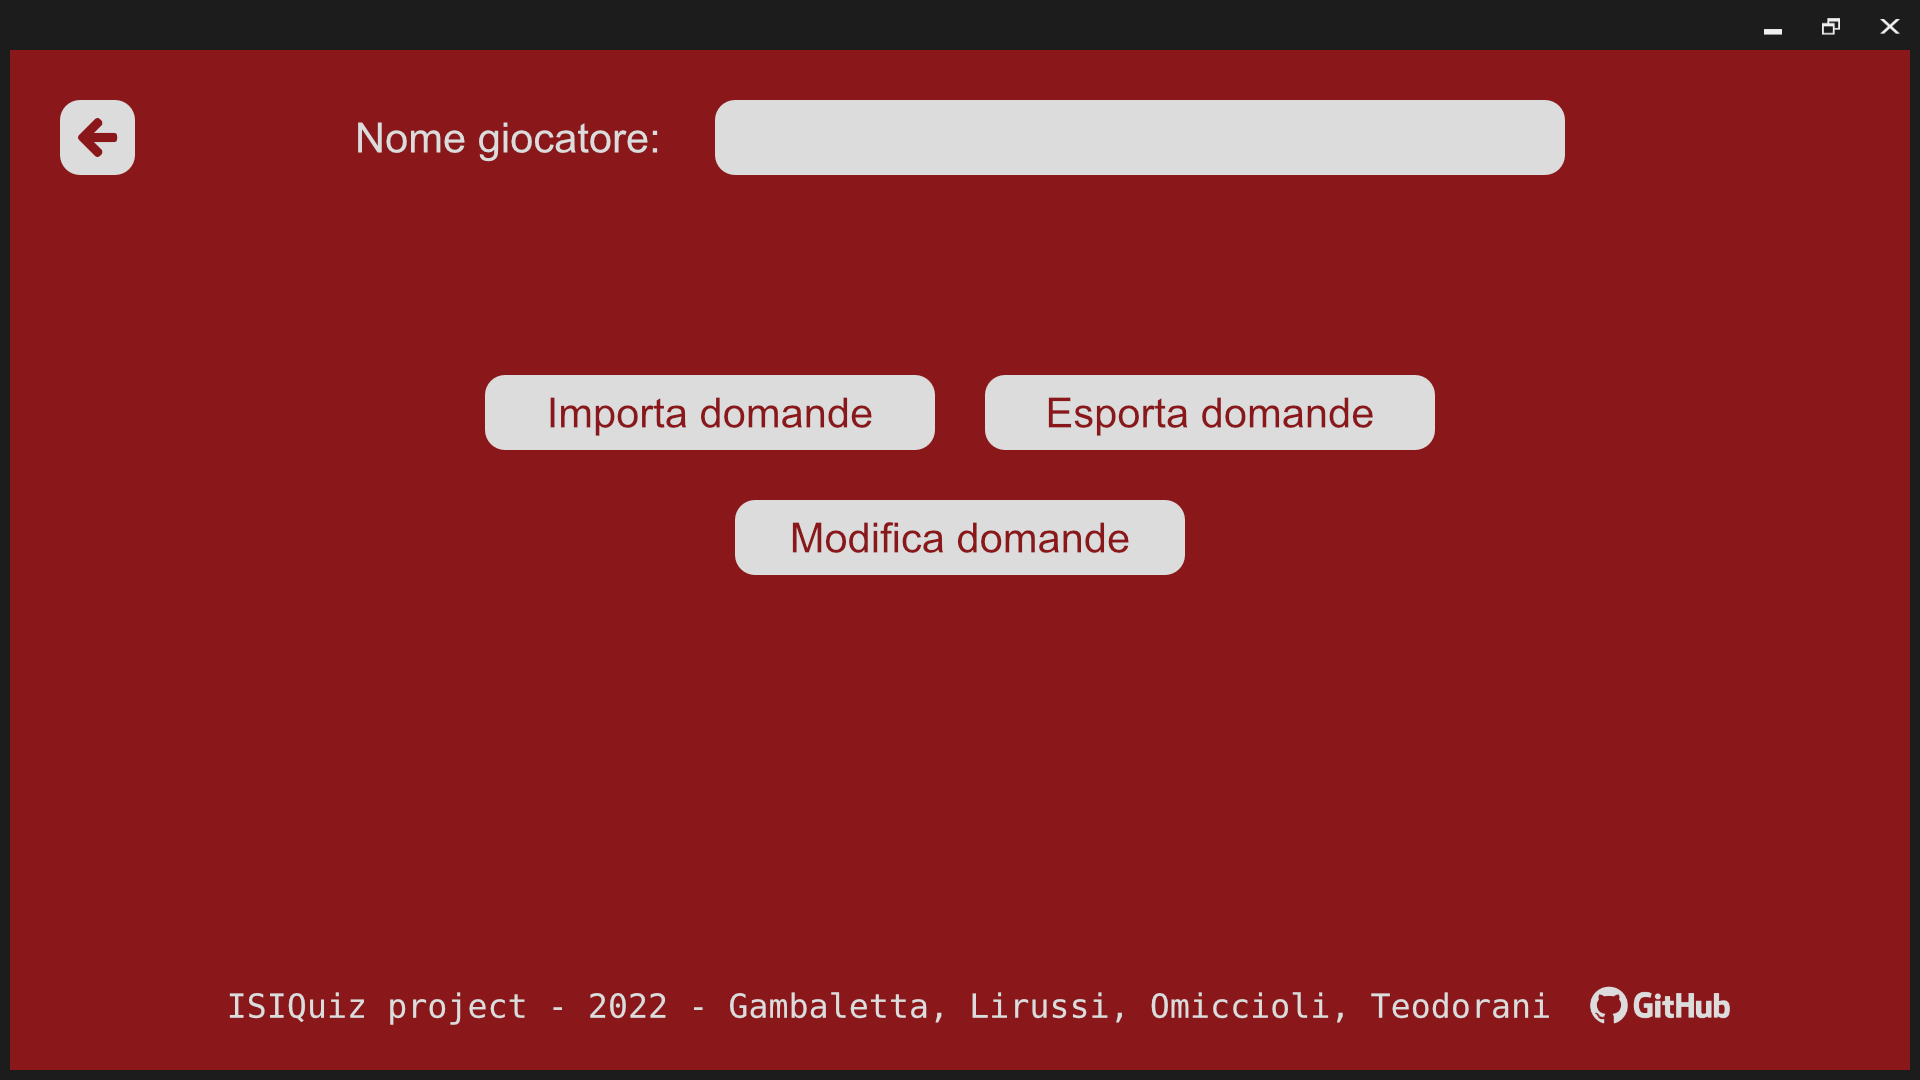
\includegraphics[width=\textwidth]{Images/mockup/settings3.png}
            \caption{Impostazioni generali}
            \label{fig:settings3}
          \end{minipage}
        \end{figure}

        \begin{figure}[H]
          \centering
          \begin{minipage}[b]{0.48\textwidth}
            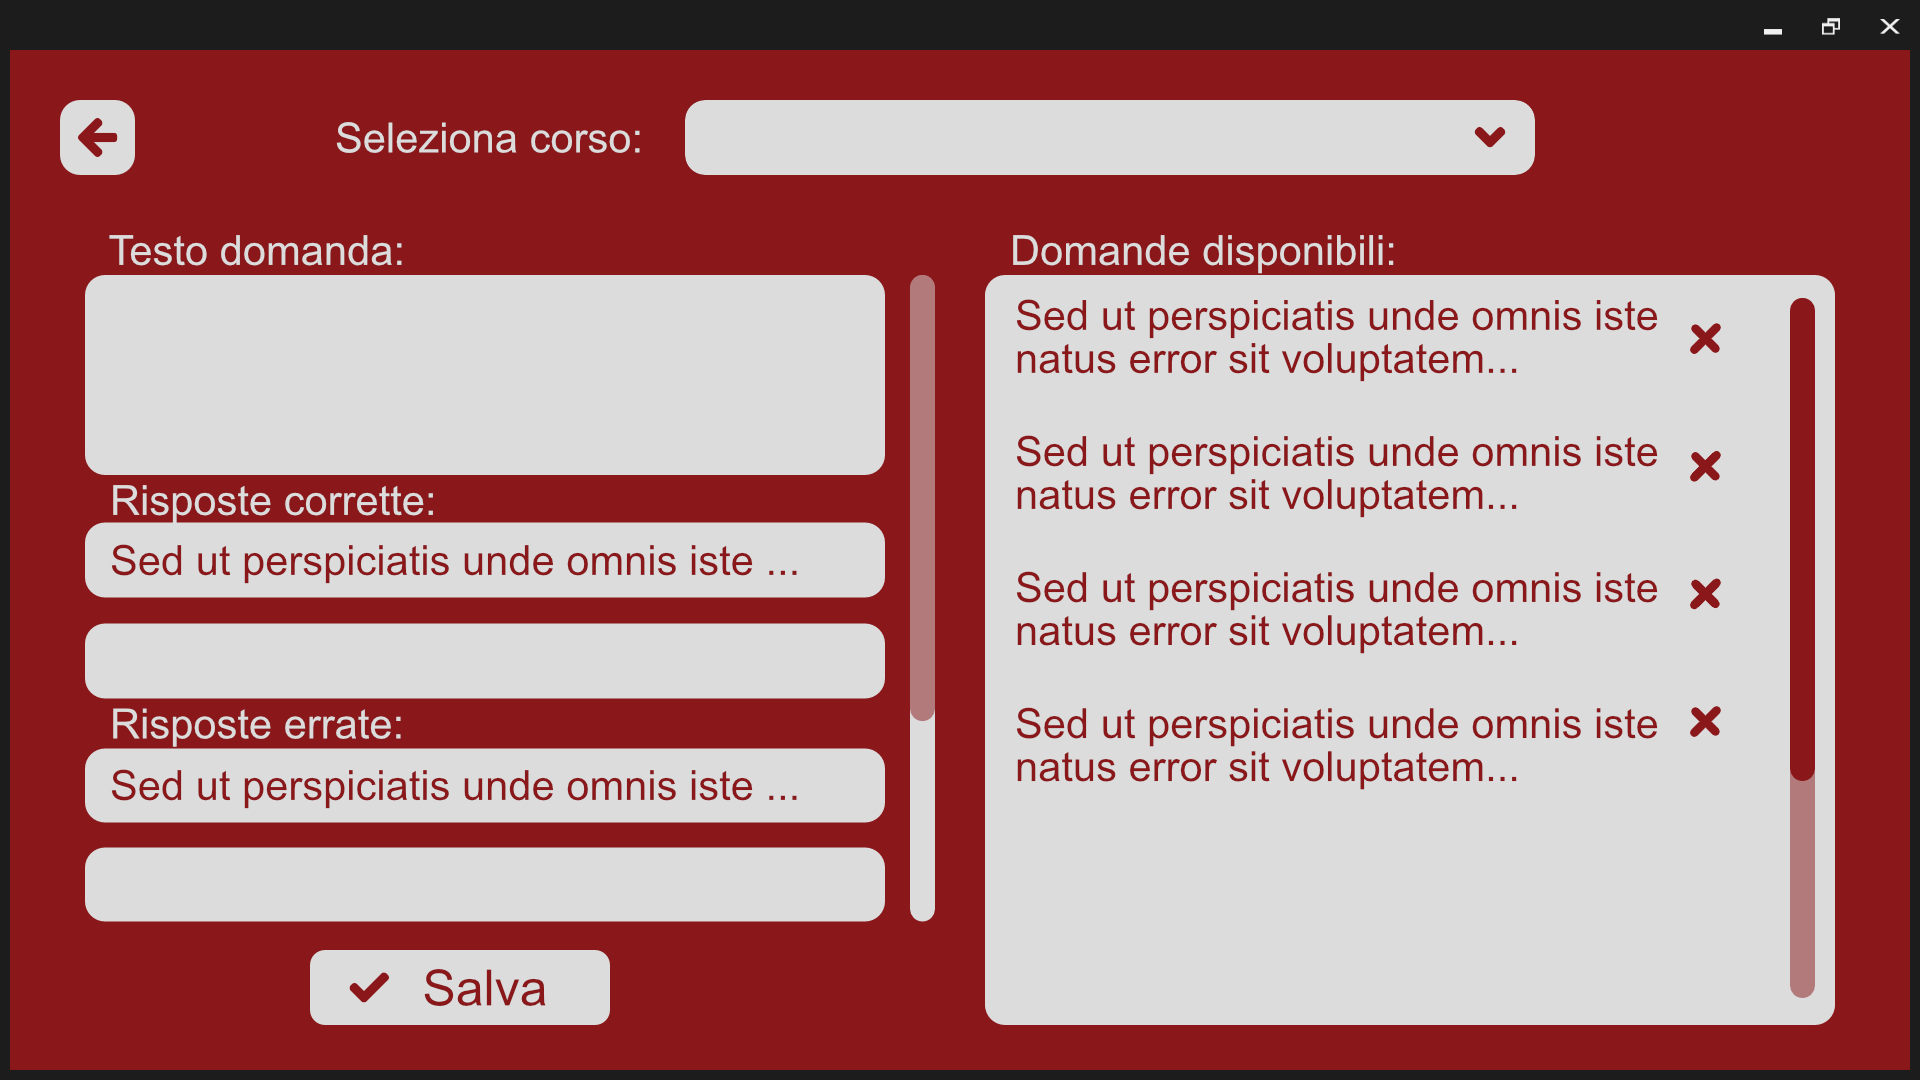
\includegraphics[width=\textwidth]{Images/mockup/import3.png}
            \caption{Inserimento di nuove domande e relative risposte per un determinato corso}
            \label{fig:import3}
          \end{minipage}
          \hfill
          \begin{minipage}[b]{0.48\textwidth}
            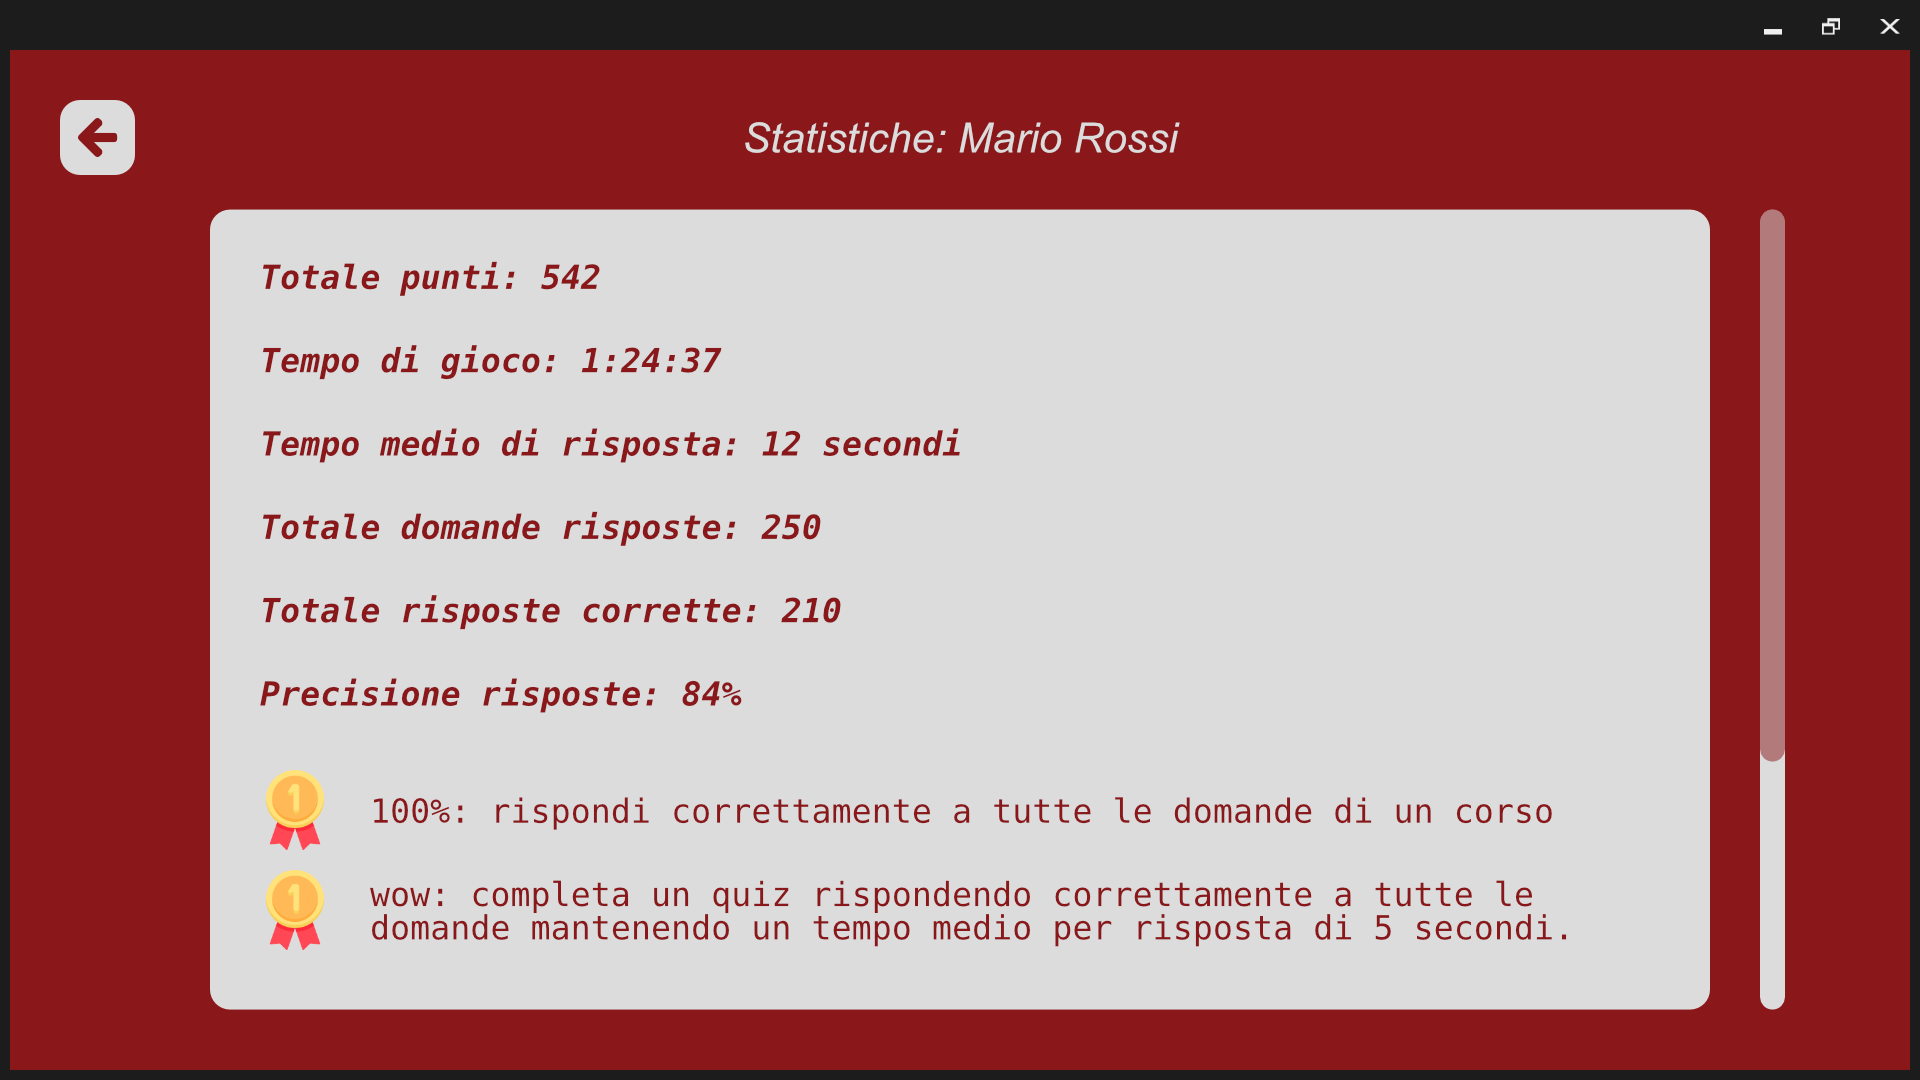
\includegraphics[width=\textwidth]{Images/mockup/achievements3.png}
            \caption{Statistiche di gioco e obiettivi raggiunti}
            \label{fig:achievements3}
          \end{minipage}
        \end{figure}

        \begin{figure}[H]
            \centering
            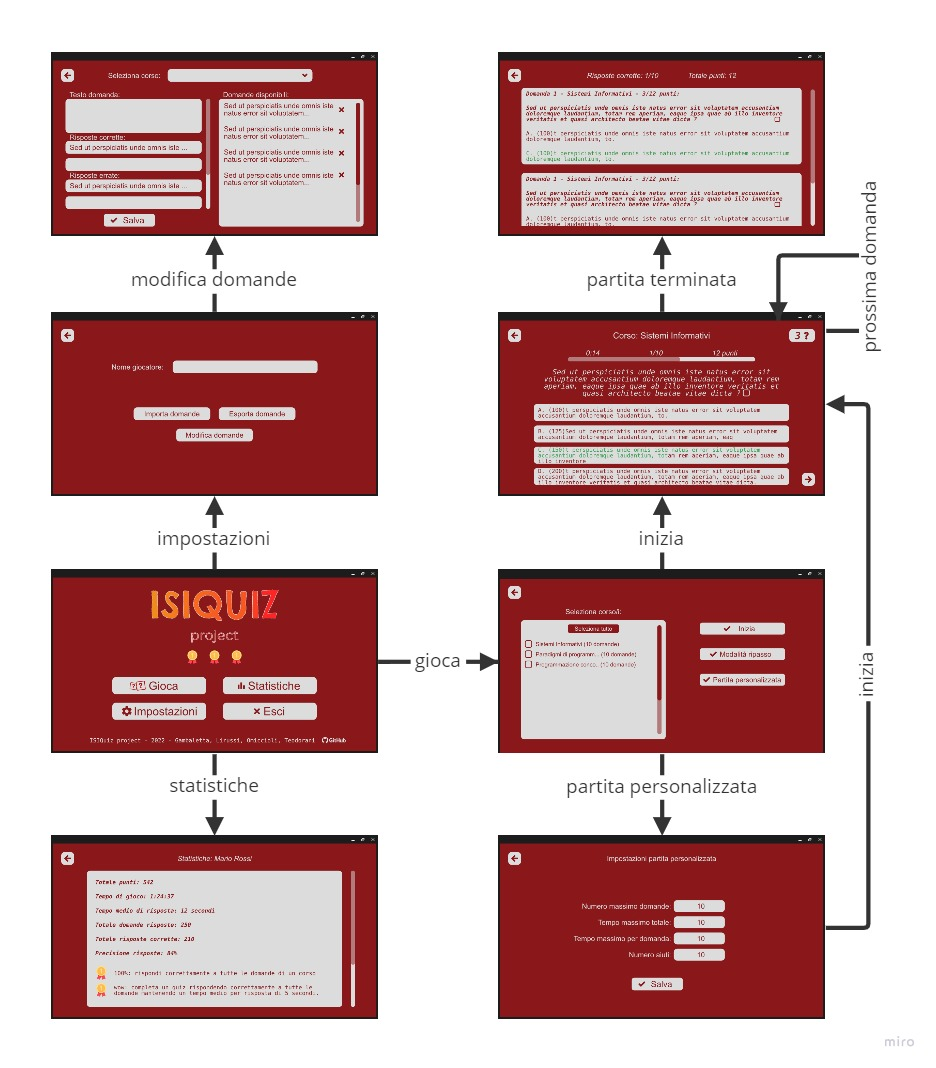
\includegraphics[width=\textwidth]{Miro/mockup_navigation.jpg}
            \caption{Tutti i mockup dell'applicazione con navigazione tra le pagine}
            \label{fig:mockup_nav}
        \end{figure}
	    
\section{Requisiti Funzionali} 
        \subsection{Obbligatori}
        All’interno di ogni partita, vengono presentate all’utente diverse domande di natura accademica, ognuna delle quali viene accompagnata da un numero predeterminato di risposte possibili, alcune corrette ed altre sbagliate. L’utente dovrà individuare le risposte corrette in un tempo massimo per non fallire la domanda. 

        \begin{enumerate}
            \item \textbf{Modalità di gioco generale}: domande a scelta multipla su tutti i corsi disponibili: al giocatore verranno poste N domande scelte casualmente tra tutti i corsi disponibili nel gioco. Ogni domanda dovrà essere risposta in T tempo massimo altrimenti verrà considerata errata.
            
            \item \textbf{Modalità di gioco materie a scelta}: domande a scelta multipla su più materie scelte dal giocatore: domande a scelta multipla su alcuni dei corsi scelti dal giocatore tra tutti i corsi disponibili: al giocatore verranno poste N domande scelte casualmente tra tutti i corsi selezionati. Ogni domanda dovrà essere risposta in T tempo massimo altrimenti verrà considerata errata.
            
            \item \textbf{Modalità di gioco materia specifica}: domande a scelta multipla su una materia scelta dal giocatore: domande a scelta multipla su un corso scelto dal giocatore tra tutti i corsi disponibili: al giocatore verranno poste N domande scelte casualmente tra quelle disponibili per il corso. Ogni domanda dovrà essere risposta in T tempo massimo altrimenti verrà considerata errata.

            \item \textbf{Interfaccia grafica} (CLI e poi JavaFX): visualizzazione menu principale, visualizzazione della domanda e di 4 possibili risposte da scegliere durante il gioco, visualizzazione dei risultati post partita. La prima iterazione del programma dovrà fornire una semplice interfaccia grafica che permetta di interagire con le funzionalità principali del gioco scrivendo le operazioni da eseguire tramite il terminale.
                \begin{enumerate}
                    \item Menu principale: la prima pagina che verrà mostrata all'avvio
                        \begin{enumerate}
                            \item Pulsante "inizia a giocare" > pagina inizia a giocare
                            \item Pulsante "statistiche e achievement" > pagina statistiche
                            \item Pulsante "impostazioni" > pagina impostazioni
                            \item Pulsante "esci" > termina l'applicazione
                        \end{enumerate}
                    \item Pagina statistiche: contiene informazioni sulle statistiche relative alle partite concluse e agli achievement raggiunti
                        \begin{enumerate}
                            \item Totale domande risposte
                            \item Totale domande risposte correttamente
                            \item Totale domande risposte sbagliate
                            \item Percentuale risposte corrette
                        \end{enumerate}
                    \item Pagina impostazioni: permette di editare le domande e le risposte oltre a salvarle ed importarle da file
                        \begin{enumerate}
                            \item Casella di testo con il quale editare lo username del giocatore ?
                            \item Form per editare le domande
                            \item Pulsante per salvare (esportare) nuove domande > salva su file le domande di un corso
                            \item Pulsante per importare nuove domande > permette di selezionare un file contenente le domande di un corso 
                        \end{enumerate}
                    \item Pagina selezione corsi: permette di selezionare prima di iniziare la partita i corsi dai quali devono essere prese le domande ed alcune impostazioni di gioco
                        \begin{enumerate}
                            \item Selezione corsi disponibili
                            \item Selezione tempo per risposta
                            \item Selezione tempo totale
                            \item Selezione numero domande della partita
                            \item Selezione numero di aiuti
                        \end{enumerate}
                    \item Pagina riepilogo post partita: permette di visualizzare il punteggio ottenuto nella partita appena conclusa e una lista con il riepilogo di tutte le domande con un'indicazione sulla correttezza della risposta data e, in caso di risposta errata, la risposta corretta corrispondente
                    \begin{enumerate}
                        \item Testo con punteggio della partita
                        \item Lista domande della partita con risposta scelta ed eventualmente risposta corretta
                    \end{enumerate}
                \end{enumerate}
            
            \item \textbf{Punteggio finale} del quiz appena effettuato: al termine della partita verrà visualizzato il punteggio ottenuto dal giocatore in base al numero di risposte corrette o errate date nella partita conclusa. (Il punteggio verrà calcolato sommando i punti relativi ad ogni domanda risposta correttamente? Se vengono utilizzati degli aiuti il punteggio cala?)
            
            \item \textbf{Visualizzazione e salvataggio delle statistiche personali}: in specifico le statistiche personali includono:
                \begin{enumerate}
                    \item Totale domande risposte
                    \item Totale risposte corrette
                    \item Totale risposte errate
                    \item Percentuale di correttezza delle risposte
                    \item Punteggio totale giocatore
                \end{enumerate}
            
            \item \textbf{Più risposte giuste} e sbagliate per ogni domanda in modo da avere una rotazione tra le possibili scelte: ogni domanda dovrà necessariamente avere almeno 3 risposte errate ed 1 corretta ma potrebbe averne a disposizione un numero superiore, da scegliere poi casualmente durante il gioco. In ogni caso dovrà essere rispettato il vincolo di avere 3 risposte errate ed 1 corretta per ogni domanda durante la partita.
            
            \item Aggiunta di \textbf{nuove domande e risposte da parte dell’utente}:
                \begin{enumerate}
                        \item Aggiunta di una nuova materia
                        \item Aggiunta di una nuova domanda
                        \item Aggiunta di 3 o più risposte errate relative ad una domanda
                        \item Aggiunta di 1 o più risposta corretta relativa ad una domanda
                        \item Aggiunta di un punteggio per una domanda
                    \end{enumerate}
        \end{enumerate}  

    
        \subsection{Opzionali} \label{chap:req_non_funzionali}
        \begin{itemize}
            \item \textbf{Sfida a tempo}: rispondere a più domande possibili in un intervallo di tempo limitato
            \item \textbf{Aiuti su richiesta}: all’utente vengono messi a disposizione un numero specifico di aiuti ad ogni partita con i quali semplificare la scelta della risposta. Utilizzando uno degli aiuti verrà eliminata una tra le risposte errate, semplificando così la scelta. Potranno essere utilizzati al massimo 2 aiuti per ogni domanda. (Il numero di aiuti a disposizione sarà configurabile dall'utente prima di iniziare una partita?)
            \item \textbf{Revisione solo delle risposte sbagliate}: l’utente può scegliere una modalità di gioco in cui ripassare esclusivamente le domande precedentemente sbagliate
            \item \textbf{Medaglie-achievement} quando si completano delle sfide (es. più punti di un certo limite, più giornate continuativamente, aver risposto bene a tutte le domande di una materia)
            \item Salvataggio delle statistiche relative al tempo medio di risposta e tempo totale di gioco
        \end{itemize}
	\section{Requisiti Non Funzionali}
        \begin{itemize}
            \item Interfaccia grafica intuitiva e che fornisca feedback coerenti all'utente per comunicargli lo stato delle sue azioni (ad esempio indicando con colore verde e checkmark una risposta qualora essa sia corretta)
            \item Interfaccia grafica accessibile agli utenti daltonici
            \item Interfaccia grafica reattiva: alle azioni di un utente devono corrispondere degli aggiornamenti dell'interfaccia stessa in tempi ragionevoli per non rovinare la user experience
            \item Realizzare un sistema modulare che permetta estensioni future (ad esempio uno sviluppo distribuito che permetta di realizzare funzionalità di gioco multiplayer)
            \item Il sistema dovrà essere in grado di memorizzare dati di interesse in maniera consistente
            \item Il sistema deve essere funzionante in diversi sistemi operativi nei quali è installata una appropriata Java Virtual Machine (il requisito minimo considera il funzionamento su sistemi Windows, Linux e MacOS).
            \item Il sistema deve essere fault-tolerant, cioè deve continuare a funzionare in modo affidabile e deve essere privo di falle che permettano al giocatore di barare.
        
        \end{itemize}

\section{Requisiti Implementativi}
        \begin{itemize}
            \item Linguaggio di programmazione Scala versione 3.2.0
            \item Scala FX 19.0.0 per l'interfaccia grafica
            \item Utilizzo di JDK X ?
            \item Per il salvataggio delle domande e delle relative risposte deve essere utilizzata la notazione JSON in modo che l'integrazione con il software possa utilizzare librerie generiche già disponibili.
            \item Per lo sviluppo dovrà essere utilizzato l'IDE IntelliJ in modo da avere consistenza tra i membri del team di sviluppo.
        \end{itemize}

	
    % -*- root: ../main.tex -*-

% Devono essere esposte le scelte progettuali operate nelle varie fasi di sviluppo dell'elaborato. In questa sezione devono essere documentati gli schemi di progetto relativamente all'architettura complessiva del sistema e alle sue componenti di rilievo che possano meritare un'analisi di dettaglio. Per le componenti software si può ricorrere ad esempio a diagrammi delle classi, di sequenza, stato, attività. Per le componenti hardware è possibile includere opportuni schemi in grado di descrivere l'architettura fisica adottata.
% 15000 - 24000 battute 

%Architettura complessiva, descrizione di pattern architetturali usati, componenti del sistema distribuito, scelte tecnologiche cruciali ai fini architetturali -- corredato da pochi ma efficaci diagrammi
%Ricordate che una scelta architetturale può ritenersi giustificata o meno solo a fronte dei requirement che avete indicato; viceversa, ogni requirement "critico" dovrebbe influenzare qualcuna della scelte architetturali effettuate e descritte.
%L'architettura deve spiegare quali sono i sotto-componenti del sistema (da 5 a 15, diciamo), ognuno cosa fa, chi parla con chi e per dirsi cosa -- i diagrammi aiutano, ma poi la prosa deve chiaramente indicare questi aspetti.
\chapter{Design Architetturale}
    ...
    \section{Architettura Generale}
    Inserimento del diagramma delle classi generale in cui si vedono le interazioni tra Model View e Controller
    
    \begin{figure}[H]
        \centering
        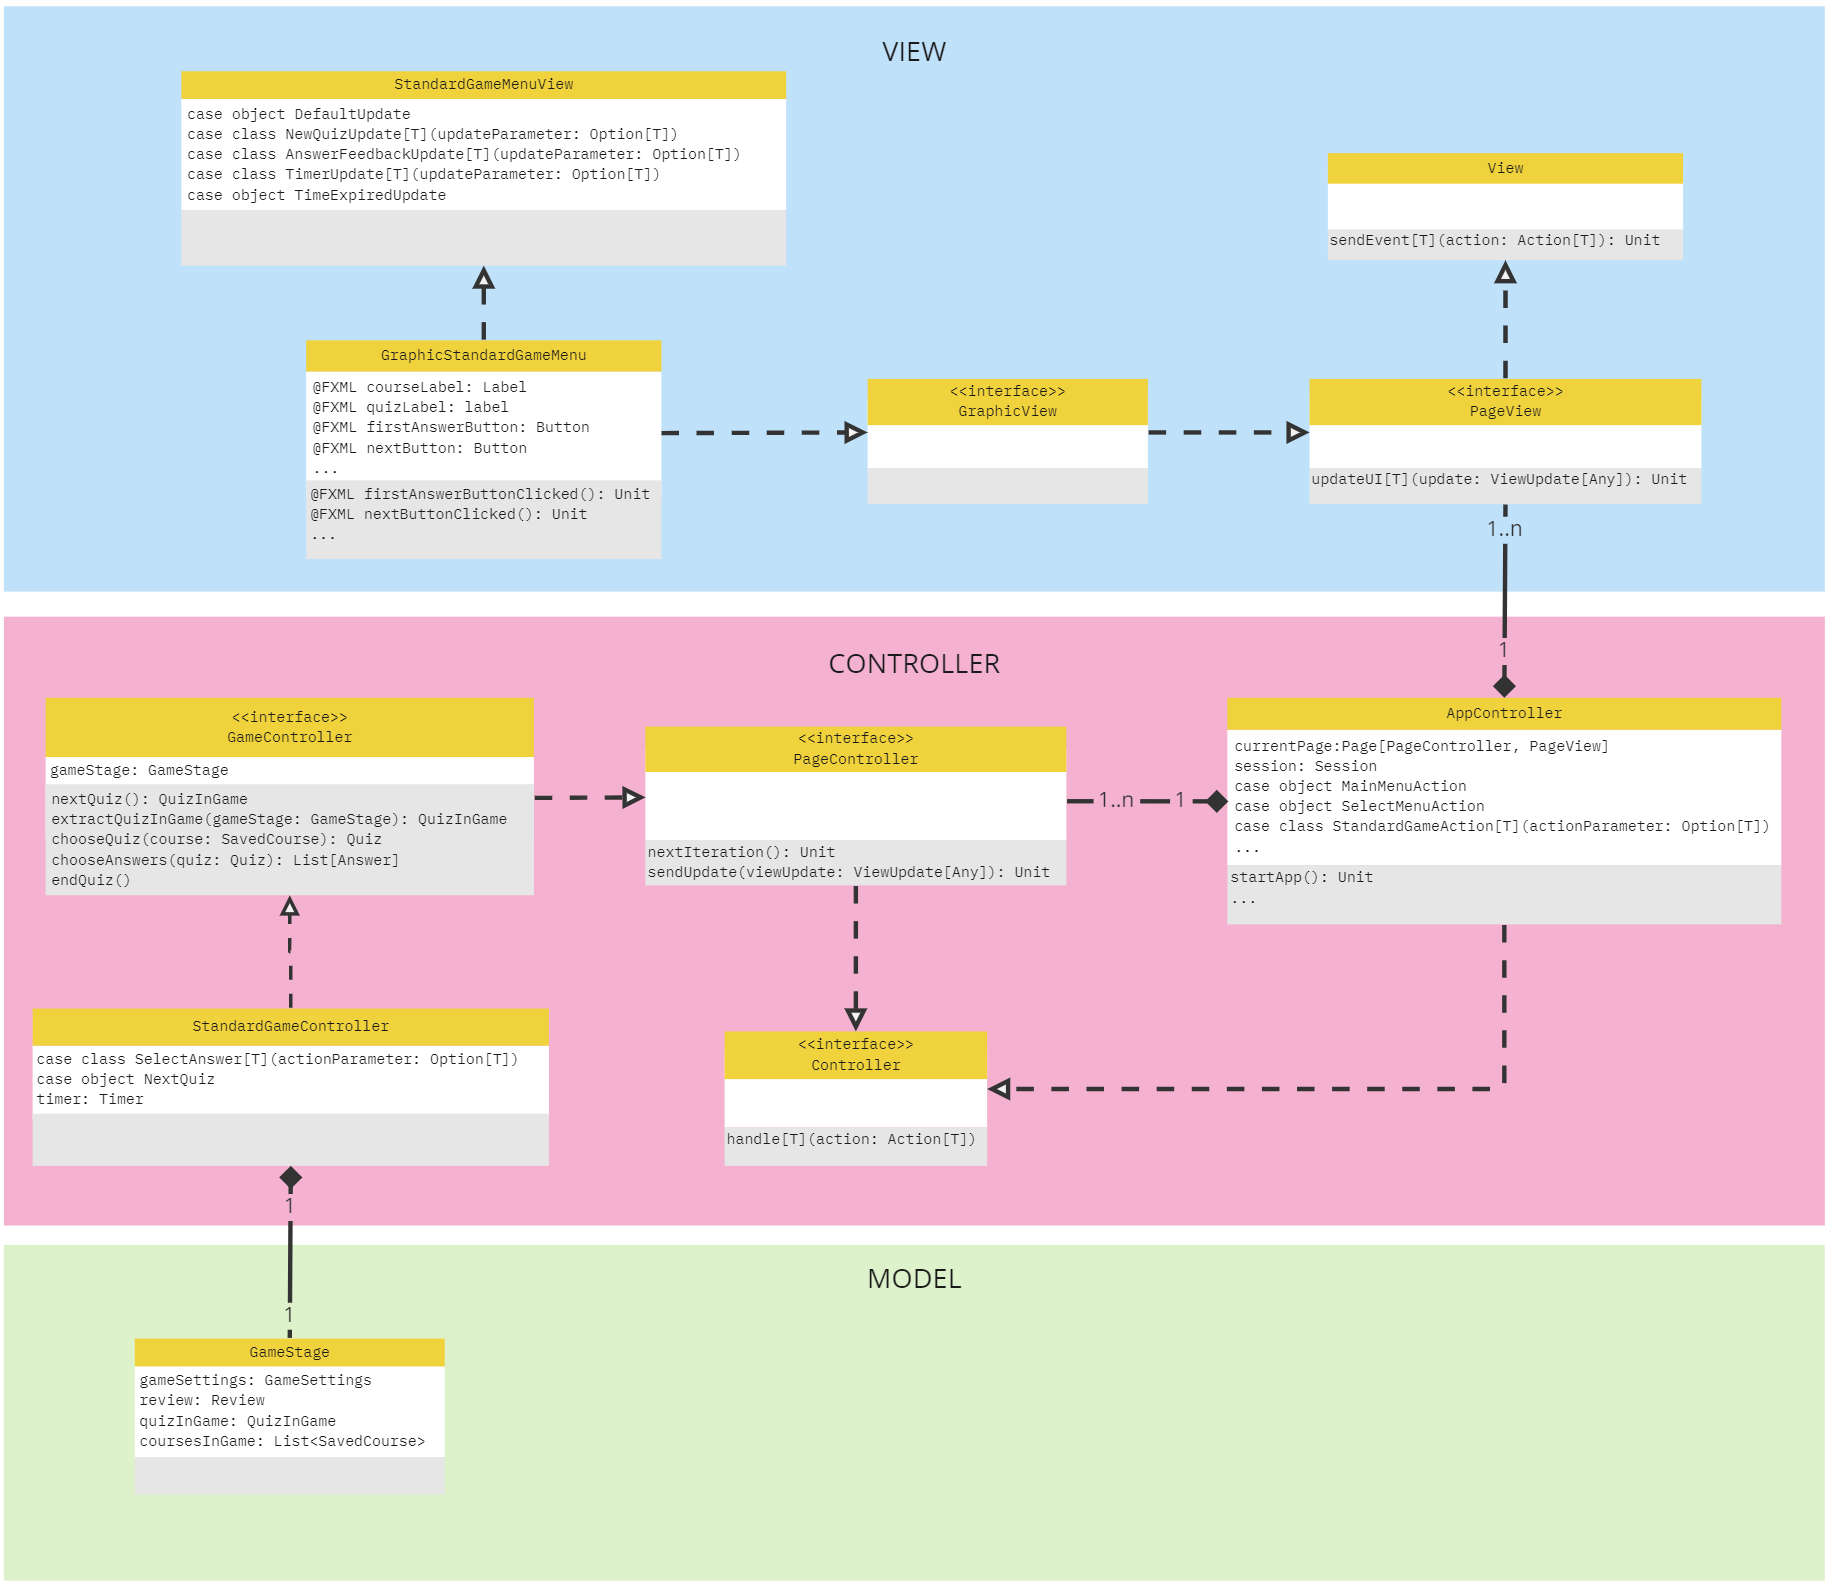
\includegraphics[width=\textwidth]{Miro/general_architecture.png}
        \label{fig:Sprint9BL2}
    \end{figure}
    
    \section{Pattern Architetturali Utilizzati}
        Nel sistema è stato utilizzato il pattern Model View Controller (MVC) in modo da modularizzare quanto più possibile le parti relative all'interfaccia grafica, la modellazione e la logica dell'applicazione. 
        Questo pattern è stato utile considerando anche la metodologia di sviluppo agile per realizzare versioni successive del sistema implementando, ad esempio, un'interfaccia basata su linea di comando nelle prime fasi del progetto e poi una interfaccia che utilizzasse JavaFX nelle fasi successive di sviluppo.
        
        Il funzionamento del pattern MVC è il seguente:
        \begin{itemize}
            \item Il Model fornisce i metodi per accedere ai dati;
            \item La View si occupa di interagire con l'utente, notificare il Controller e visualizzare i dati del Model;
            \item Il Controller riceve i comandi dell'utente e si occupa di aggiornare lo stato della View e del Model.
        \end{itemize}
    
    % -*- root: ../main.tex -*-
%Scelte rilevanti, pattern di progettazione, organizzazione del codice -- corredato da pochi ma efficaci diagrammi
%Il design di dettaglio "esplode" (dettaglia) l'architettura, ma viene concettualmente prima dell'implementazione, quindi non metteteci diagrammi ultra-dettagliati estratti dal codice, quelli vanno nella parte di implementazione eventualmente.
\chapter{Design di Dettaglio}\label{chap:design}
In questo capitolo, partendo dal design architetturale sopra descritto, verrà analizzata in dettaglio la struttura del sistema descrivendo le caratteristiche dei componenti e la relazione che c'è tra loro.

View: factory;
model: spiegazione della gestione quiz - review e game settings generalizzate
controller

    \section{Model}
    Inserimento del diagramma delle classi del Model
        \begin{itemize}
            \item 
            \item 
            \item 
        \end{itemize}
    \section{View}
    Inserimento del diagramma delle classi della View.
    
    Per scegliere il colore primario del sito e il colore del testo sovrastante, si è utilizzato \href{https://m2.material.io/resources/color/#!/?view.left=1&view.right=1&primary.color=8a171a&secondary.color=DEDEDE}{Material Design - Color Tool}, così che avessero il giusto contrasto e, per controllare che veramente soddisfacessero le \textit{WCAG (Web Content Accessibility Guidelines)}, è stato utilizzato \href{https://webaim.org/resources/contrastchecker/?fcolor=DEDEDE&bcolor=8A171A}{WebAIM}.
    
    \section{Controller}
    Inserimento del diagramma delle classi del Controller
    % -*- root: ../main.tex -*-

% Esporre i principali problemi affrontati durante l'effettiva realizzazione delle componenti hardware/software e illustrare le soluzioni implementative adottate. Se l'elaborato ha previsto l'utilizzo di tecnologie già disponibili sul mercato, discuterne brevemente le caratteristiche e motivarne l'adozione rispetto ad altre soluzioni assimilabili. NOTA: in questa sezione devono essere riportate esclusivamente le porzioni di codice ritenute particolarmente significative. 
% 10000 - 21000 battute
%per ogni studente, una sotto-sezione descrittiva di cosa fatto/co-fatto e con chi, e descrizione di aspetti implementativi importanti non già presenti nel design
\chapter{Implementazione}\label{chap:impl}
Nell'implementazione non ci sono aspetti particolari da segnalare in quanto lo sviluppo del codice ha seguito piuttosto fedelmente quanto deciso nel design del sistema. Si riportano quindi, per ogni membro del team, i principali componenti implementati ed i ruoli assunti durante il progetto.

\section{Gambaletta Daniele}
    All'interno del progetto ho ricoperto il ruolo di \textbf{domain expert}, quindi sono stato intervistato all'inizio per capire i requisiti dell'applicativo, ho controllato i mockup e li ho fatti correggere in base ai miei gusti personali, ho controllato che venissero rispettate le mie indicazioni durante lo sviluppo e dato feedback finali (presenti nel capitolo \ref{conclusioni}) una volta che è stata rilasciata la versione definitiva.
    
    Model
    \begin{itemize}
        \item Session
        \item PlayerStats
        \item SavedCourse
        \item InGamePlayerStats in GameStage
    \end{itemize}

    Utils
    \begin{itemize}
        \item Json Parser
        \item Storage Handler
    \end{itemize}
    
    Controller
    \begin{itemize}
        \item contributi in AppController con l'aggiunta della Session
    \end{itemize}

    FXML
    \begin{itemize}
        \item statistics
    \end{itemize}
    
\section{Lirussi Igor}
    Ho svolto il compito di gestire il progetto dal punto di vista della metodologia Scrum facendo lo \textbf{scrum master}. Ho controllato durante tutte le fasi del progetto che utilizzassimo correttamente i principi scelti del lavoro agile, controllando e sistemando le issue, gli sprint e il product backlog.

    FXML struttura
    \begin{itemize}
        \item add course menu
        \item add quiz menu
        \item edit course menu
        \item edit quiz menu
        \item review - grafica
    \end{itemize}

    Controller
    \begin{itemize}
        \item Add course menu
        \item Add quiz menu
        \item Edit course menu
        \item Edit quiz menu
    \end{itemize}
    
\section{Omiccioli Riccardo}
   In qualità di \textbf{product owner} del progetto ho: presieduto i vari meeting svolti dal team di sviluppo, identificato i requisiti principali (raffinati poi con il team) dell'applicativo richiesto e organizzato il lavoro del team. Il mio lavoro si è principalmente concentrato nel design e realizzazione dell'architettura generale dell'applicazione implementando, in particolare, la parte relativa ai \textit{controller}, alle \textit{view} e alla comunicazione tra essi.
   
    FXML:
    \begin{itemize}
        \item Add course menu - in collaborazione con Lirussi
        \item Add quiz menu - in collaborazione con Lirussi
        \item Blitz game
        \item Custom menu
        \item Default menu
        \item Edit course menu - in collaborazione con Lirussi
        \item Edit quiz menu - in collaborazione con Lirussi
        \item Main menu
        \item Review menu - in collaborazione con Lirussi
        \item Select menu - in collaborazione con Teodorani
        \item Standard game - in collaborazione con Teodorani
    \end{itemize}
    Controller:
    \begin{itemize}
        \item Package actions
        \item App controller
        \item Blitz game controller
        \item Controller
        \item Custom menu controller
        \item Game controller - in collaborazione con Teodorani
        \item Main menu controller
        \item Standard game controller - in collaborazione con Teodorani
        \item Select menu controller - in collaborazione con Teodorani
    \end{itemize}
    Model:
    \begin{itemize}
        \item Game settings
        \item Game stage - in collaborazione con Gambaletta, Lirussi e Teodorani
        \item Timer
    \end{itemize}
    View:
    \begin{itemize}
        \item Blitz game menu
        \item Blitz view
        \item Custom menu
        \item Default menu
        \item Main menu - in collaborazione con Teodorani
        \item Main menu view - in collaborazione con Teodorani
        \item Select menu - in collaborazione con Teodorani
        \item Select menu view - in collaborazione con Teodorani
        \item Standard game menu
        \item Package updates
        \item View - in collaborazione con Teodorani
    \end{itemize}
    Altro:
    \begin{itemize}
        \item Main
    \end{itemize}
    
\section{Teodorani Cecilia}
    Insieme ad Omiccioli, ho seguito lo sviluppo generale dell'architettura, realizzando alcuni \textit{controller}, \textit{view} e componenti del \textit{model}. Di quest'ultimo mi sono anche occupata di standardizzare tutto il codice al termine dell'implementazione del progetto. In più, mi sono assicurata che il \textit{model} fosse adeguatamente testato, sviluppando test molto dettagliati. Infine, per quanto riguarda la GUI, ho messo a punto tecniche per la user experience e l'accessibilità. Per la prima ho adottato tecniche standard, quali ad esempio il font e la disposizione dei vari componenti nella pagina, mentre per la seconda ho utilizzato dei tool, per garantire che soddisfacessero le \textit{WCAG (Web Content Accessibility Guidelines)}. In particolare, per il colore primario del sito e il colore del testo sovrastante, si è utilizzato \href{https://m2.material.io/resources/color/#!/?view.left=1&view.right=1&primary.color=8a171a&secondary.color=DEDEDE}{Material Design - Color Tool} e \href{https://webaim.org/resources/contrastchecker/?fcolor=DEDEDE&bcolor=8A171A}{WebAIM}.
    
    FXML:
    \begin{itemize}
        \item Review Menu
        \item Select Menu - in collaborazione con Omiccioli
        \item Standard Game - in collaborazione con Omiccioli
    \end{itemize}
    Controller:
    \begin{itemize}
        \item Select Menu Controller - in collaborazione con Omiccioli
        \item Game Controller - in collaborazione con Omiccioli
        \item Standard Game Controller - in collaborazione con Omiccioli
    \end{itemize}
    Model:
    \begin{itemize}
        \item Answer
        \item Game Stage - in collaborazione con Gambaletta, Lirussi e Omiccioli
        \item Course Identifier - in collaborazione con Gambaletta
        \item Quiz - in collaborazione con Gambaletta
        \item SavedCourse - in collaborazione con Gambaletta
        \item Session - in collaborazione con Gambaletta
    \end{itemize}
    View (realizzata la struttura di tutti gli update in \textit{nomeFile}MenuView sotto riportati, mentre dei controller grafici \textit{nomeFile}Menu la struttura generale e la navigazione tra le varie pagine):
    \begin{itemize}
        \item Add Course Menu - in collaborazione con Lirussi
        \item Add Course Menu View - in collaborazione con Lirussi
        \item Add Quiz Menu - in collaborazione con Lirussi
        \item Add Quiz Menu - in collaborazione con Lirussi
        \item Custom Menu
        \item Custom Menu View - in collaborazione con Omiccioli
        \item Main menu - in collaborazione con Omiccioli
        \item Main Menu View - in collaborazione con Omiccioli
        \item Select Menu - in collaborazione con Omiccioli
        \item Select Menu View - in collaborazione con Omiccioli
        \item Settings Menu View - in collaborazione con Gambaletta, Lirussi
        \item Standard Game Menu - in collaborazione con Omiccioli
        \item Statistics Menu View - in collaborazione con Gambaletta
        \item View - in collaborazione con Omiccioli
    \end{itemize}

    
    % -*- root: ../main.tex -*-

% Esporre lo stato di funzionamento effettivo del sistema progettato ad elaborato concluso. Per ciascuna delle funzionalità salienti devono essere tabellate e discusse le performance riscontrate mediante opportuni test eseguiti in fase di validazione del progetto. I tempi di esecuzione/comunicazione devono essere accompagnati dalle caratteristiche dell'hardware sul quale è eseguito il software. Qualora l'elaborato includa algoritmi innovativi, indicarne la complessità computazionale (avendo cura di esporre lo pseudo codice nella sezione Implementazione).
% 3000 - 6000 battute

\chapter{Testing e Performance}
 ... non so se volgiamo farlo, ma forse un due righe non guastano
    % -*- root: ../main.tex -*-
\chapter{Retrospettiva}

\section{Svolgimento}
Gli sprint sono stati portati avanti nel seguente modo:
    \paragraph{Sprint Planning}
        Pianificazione a inizio sprint degli obiettivi, tempistiche e responsabilità nel periodo dello sprint corrente. Diviso in due parti:
        \begin{itemize}
        \item\textbf{parte 1} 
            Viene raffinato e rivisto il product backlog, viene effettuata la scelta dello sprint goal (what).
        \item\textbf{parte 2}
            Si decidono gli item e viene raffinato come implementarli (how). Effettuato con solo il team senza la figura del product owner
        \end{itemize}
    \paragraph{[Iterativo] Daily scrum} Breve meeting svolto giornalmente. Viene utilizzato per gli aggiornamenti sull'andamento del progetto, senza scendere nei dettagli implementativi.
    \paragraph{[Occasionale] Pair Programming } Utilizzato per risolvere problemi che causano il blocco di un componente del team per parecchio tempo su una issue.
    \paragraph{Meeting finale}
        Riflessioni e considerazioni finali sullo spint passato. Suggerimenti per migliorare il prossimo. Diviso in tre parti: 
        \begin{itemize}
        \item\textbf{Product backlog refinement} aggiunta di dettagli e riordino del product backlog
        \item\textbf{Sprint review} è stato ispezionato l'incremento, il Minimum Viable Product o di risultati sul processo. Discernere cosa è stato fatto e cosa no
        \item\textbf{Retrospettiva} Considerazioni sul team stesso e sui miglioramenti per il prossimo sprint. 
        \end{itemize}

% NOTA: le parti qui sotto sono prese dalla cartella "process", all'interno dei vari sprint, solo la "sprint review" di ognuno
\section{Sprint 1}
    \section{Sprint 1 Review}
%only this part is present also in the main report
Durante questo primo sprint abbiamo completato l'organizzazione di massima.
\paragraph{Deliverables} 
I deliverables per questo sprint sono stati i seguenti:
\begin{itemize}
    \item Intervista con il cliente corredata da domande
    \item Ubiquitous Language
    \item Setup Organizzazione GitHub
    \item Setup Report, con relativa repository e CI
\end{itemize}

    
\section{Sprint 2}
    \section{Sprint 2 Review}
%only this part is present also in the main report
Durante questo sprint abbiamo realizzato l'analisi dei requisiti del sistema e ideata l'architettura generale del sistema, dalla quale sono sorti alcuni dubbi che sono stati poi discussi e chiariti con l'esperto del dominio. Sono state realizzare due versioni dei mockup dell'applicazione, le quali hanno ricevuto entrambe giudizi positivi, ma andranno successivamente unite e raffinate per soddisfare al meglio i requisiti del committente.
\paragraph{Deliverables} 
I deliverables per questo sprint sono stati i seguenti:
\begin{itemize}
    \item Mockup
    \item Diagramma dei casi d'uso
    \item Diagramma delle classi
\end{itemize}

    
\section{Sprint 3}
    \section{Sprint 3 Review}
%only this part is present also in the main report
Abbiamo studiato/implementato...
\paragraph{Deliverables} 
obiettivi raggiunti
\begin{itemize}
    \item uno
    \item due
    \item tre
\end{itemize}


\section{Sprint 4}
    %only this part is present also in the main report.
Durante questo sprint è stata implementata completamente la visualizzazione della pagina iniziale, è stata implementata la risposta di un quiz ed è stato effettuato il setup della CI.
\paragraph{Deliverables} 
I deliverables per questo sprint sono stati i seguenti:
\begin{itemize}
    \item Visualizzazione della pagina iniziale
    \item Implementata risposta di un quiz
    \item Setup della CI 
\end{itemize}


    % -*- root: ../main.tex -*-

% Esporre brevemente le considerazioni conclusive sul progetto presentato, indicando anche i possibili sviluppi futuri.
% 1500 - 3000 battute

\chapter{Conclusioni}\label{conclusioni}

    \section{Sviluppi Futuri}
    Tutti i requisiti funzionali opzionali sopra citati (capitolo \ref{chap:req_non_funzionali}) sono sicuramente i primi aspetti da inserire, dal momento che sono stati indicati dall'esperto del dominio durante l'analisi iniziale.
   In più, dato che il progetto sviluppato è un'applicazione desktop, non è difficile immaginarsi ulteriori funzionalità aggiuntive:
    
    \begin{itemize}
        \item Salvataggio di tutti i dati del giocatore e delle partite in una architettura cloud o server based: si può creare una classifica generale con tutti gli studenti, basata su quante partite hanno effettuato e quante risposte corrette hanno dato sul totale dei quiz;
    
        \item Sfida tra più studenti: in questa modalità di gioco più utenti possono sfidarsi utilizzando l'applicativo sui propri dispositivi;
        
        \item Condivisione dei quiz inseriti da un utente: chiunque può avere a disposizione ulteriori corsi e/o quiz sui quali esercitarsi, cercando di coprire il più possibile gli argomenti presenti negli esami;
        
        \item Segnalazione da parte dei giocatori di quiz da correggere, perché incompleti o inesatti.
    \end{itemize}
    
    

    
    


\nocite{*} % Includes all references from the `references.bib` file
\printbibliography[title={Bibliografia completa}]

\end{document}
